% ================================= preamble ===================================
% To compile this document on your own machine, run the following commands in
% the terminal:
%   pdflatex main
%   biber main
%   makeglossaries main
%   pdflatex main
%   pdflatex main
% In Overleaf, just click "Compile" once or CTRL-S.

% You can add options by entering text between the square brackets (`[]`).
%   Use the `noul` option if there is a conflict with the `\ul` command.
%   Use the `review` option when sending to committee members for review.
%   Use the `internal` option for a prospectus or graduate research paper.
%   Use the `style` option to customize citations: `style=ieee`.
%   Use the `dvipsnames` option to add the dvipsnames for colors.

\documentclass[style=ieee,dvipsnames]{afitthesis}
% #OPT: Fix AFIT crest
    % Missing Stars, and Eagle

% ------------------------------ Folders --------------------------------

% Define the default location to look for supporting documents.
\makeatletter
\def\input@path{{Chapters/}{Other/}{Tables/}{Figures/}
    {Chapters/C1}{Chapters/C2/}{Chapters/C3/}
    {Chapters/C2/Figures}
}
\makeatother
% Define the default location to look for figures.
\graphicspath{{Figures}{Chapters/C1/}{Chapters/C2/}{Chapters/C3/}{Chapters/C2/Figures}}
\usepackage{import} % For subimporting chapters with dedicated Figures folder

% ------------------------ Main document information ---------------------------

% NOTE: The following macros are the meta data of your document, like the title,
% author, and department. Some of these apply to the whole document. Some, like
% in the section after this, apply to the SF 298 form only. Several are
% commented out because they are probably not needed for your situation.

% #TODO: Settle on a title
\title{
    % WORKING TITLE:\\
    % Increasing Efficiency, Efficacy, and Extensibility\\
    % in Heterogeneous Agent Reinforcement Learning 
    Reducing Computational Barriers to Heterogeneous Multi-Agent Reinforcement Learning
}
\author{Brandon Hosley}
% \authorsecond{} % Use these if other students contributed.
% \authorthird{}
% \authorfourth{}
\rank{Captain, USAF}
% \ranksecond{} % Use these if other students contributed.
% \rankthird{}
% \rankfourth{}
\previousdegrees{B.Sc., M.Sc.}
\newdegree{Doctor of Philosophy in Operations Research}
\graduationdate{March 2026} % expected month and year
\department{\ENS} % \ENY, \ENG, \ENP, \ENC, \ENS, or \ENV
\doctype{Dissertation} % Default is "thesis".
\docdesignator{AFIT-ENS-DS-26-M-094} % provided by AFIT
% \address{} % Default is WPAFB.
% \disclaimer{} % Default is non-attribution of views expressed in paper to the USAF.
% \copyrightstatement{} % Default claims ownership by US government.
\committee{ % rank name, Ph.D. \\ role
    {Bruce Cox, Ph.D.\\Chair},
    {Matthew Robbins, Ph.D.\\Member},
    {Maj Nicholas Yielding, Ph.D.\\Member}}
\abstract{\begin{abstract}	
    Cool, awesome abstract that tells people why they should 
    read your awesome thesis.
\end{abstract}}
% ABSTRACT NOTE: This text should probably stay under 100
% words or so. Make sure to not put any personally-identifiable information
% about others in this text. This will be duplicated onto the SF-298 at the
% end of your thesis or dissertation. If it does not fit in the small box on
% the form, make a shorter version using the
% \texttt{\textbackslash{}sfAbstract} command.
\keywords{
    Multi-Agent Reinforcement Learning;
    Heterogeneous Agents;
    Parameter Sharing;
    Curriculum Learning;
    Implicit Indication;
    Observation Homogenization;
    Centralized Training with Decentralized Execution;
}
% #OPT: Add Dedication
%\dedication{To the one who loves me most.}
% #OPT: Add acknowledgements
%\acknowledgments

% Distribution and Control. Uncomment to specify.
% \cui{ % for Controlled Unclassified Information
%     Controlled By: AETC \\
%     Controlled By: AFIT/ENG \\
%     CUI Category(ies): PRVCY \\
%     Distribution: \DistB{CATEGORY}{DATE}{OFFICE} \\
%     POC: John Smith, 555-123-4567}
% \classified{ % for classified work
%     Classified By: \\
%     Derived From: \\
%     Declassify On: }
% \banner{cui} % automatically inserted into the header and footer

% -------------- SF 298 (Report Documentation Page) information ----------------
% #TODO: SF 298

% Necessary fields
% \sfStartDate{Sep 2023}
% \sfEndDate{Mar 2024}
% \sfContractNumber{XXXXXX-XX-X-XXXX}
% \sfGrantNumber{}
% \sfProgramElementNumber{}
% \sfProjectNumber{XXXXXXXX}
% \sfTaskNumber{}
% \sfWorkUnitNumber{}
% \sfSponsorAgency{AFXX/XXXX\\
%     Building XXX, WPAFB OH 45433-7765\\
%     DSN XXX-XXXX, COMM 937-XXX-XXXX, Email: first.last@us.af.mil }
% \sfSponsorAcronyms{}
% \sfSponsorReportNumber{}
% \sfDistribution{\DistA}
% \sfSupplementaryNotes{}
% \sfReportClassification{}
% \sfAbstractClassification{}
% \sfPageClassification{}
% \sfAbstractLimitation{UU}
% \sfResponsiblePerson{Dr. Your Advisor, AFIT/ENG}
% \sfPhoneNumber{(937) XXX-XXXX}
% \sfClassification{}

% SF 298 Override default variables
% \sfReportDate{}       % defaults to today's date
% \sfReportType{}       % defaults to \doctype{}
% \sfTitle{}            % defaults to \title{}
% \sfAuthors{}          % defaults to \author{}, \rank{}
% \sfDepartment{}       % defaults to \department{}
% \sfAddress{}          % defaults to \address{}
% \sfDocDesignator{}    % defaults to \docdesignator{}
% \sfAbstract{}         % defaults to \abstract{}
% \sfSubjectTerms{}     % defaults to \keywords{}
% \sfPageCount{}        % defaults to total number of pages

% ------------------------- Glossaries and acronyms ----------------------------

\makeglossaries%
% AF and ...
\newabbreviation{afit}{AFIT}{Air Force Institute of Technology}
\newabbreviation{asic}{ASIC}{application specific integrated circuit}
\newabbreviation{api}{API}{application programming interface}
\newabbreviation{cots}{COTS}{commercial off-the-shelf}
\newabbreviation{dod}{DoD}{Department of Defense}
\newabbreviation{darpa}{DARPA}{Defense Advanced Research Projects Agency}
\newabbreviation{isr}{ISR}{intelligence, surveillance, and reconnaissance}
\newabbreviation{kl}{KL}{Kakade-Langford}
\newabbreviation{lidar}{LIDAR}{laser imaging, detection, and ranging}
\newabbreviation[shortplural={UAS}]{uas}{UAS}{unmanned aicraft system}
\newabbreviation{sota}{SOTA}{state of the art}
\newabbreviation{offset}{OFFSET}{OFFensive Swarm-Enabled Tactics}
% DARPA

% Stochastics and Games
\newabbreviation{etdr}{ETDR}{expected total discounted reward}
\newabbreviation{mas}{MAS}{multi-agent system}
\newabbreviation{mcts}{MCTS}{Monte-Carlo tree search}
\newabbreviation[longplural={Markov decision processes}]{mdp}{MDP}{Markov decision process}
\newabbreviation{nash}{NE}{Nash equilibrium}
\newabbreviation{posg}{POSG}{partially observable stochastic game}
\newabbreviation{td}{TD}{temporal-difference}
\newabbreviation{rts}{RTS}{real time strategy}
\newabbreviation{dec-pomdp}{Dec-POMDP}{decentralised partially observable \gls{mdp}}

% General AI
\newabbreviation{ai}{AI}{artificial intelligence}
\newabbreviation{ctde}{CTDE}{centralized training with decentralized execution}
\newabbreviation{dnn}{DNN}{deep neural network}
\newabbreviation{gnn}{GNN}{graph neural network}
\newabbreviation{harl}{HARL}{heterogeneous-agent reinforcement learning}
\newabbreviation{marl}{MARL}{multi-agent reinforcement learning}
\newabbreviation{mlp}{MLP}{mulit-layer perceptron}
\newabbreviation{rl}{RL}{reinforcement learning}

% RL Algorithms
\newabbreviation{a3c}{A3C}{asynchronous advantage actor-critic}
\newabbreviation{haa2c}{HAA2C}{heterogeneous-agent \gls{a3c}}
\newabbreviation{impala}{IMPALA}{importance weighted actor-learner architecture}

\newabbreviation{maddpg}{MADDPG}{multi-agent deep-deterministic policy gradient}
\newabbreviation{haddpg}{HADDPG}{heterogeneous-agent deep-deterministic policy gradient}
\newabbreviation{ippo}{IPPO}{independent \gls{ppo}}

\newabbreviation{td3}{TD3}{twin-delayed deep-deterministic policy gradient}
\newabbreviation{matd3}{MATD3}{multi-agent \gls{td3}}
\newabbreviation{hatd3}{HATD3}{heterogeneous-agent \gls{td3}}

\newabbreviation{ppo}{PPO}{proximal policy optimization}
\newabbreviation{happo}{HAPPO}{heterogeneous-agent \gls{ppo}}
\newabbreviation{mappo}{MAPPO}{multi-agent \gls{ppo}}

\newabbreviation{trpo}{TRPO}{trust region policy optimization}
\newabbreviation{hatrpo}{HATRPO}{heterogeneous-agent \gls{trpo}}
\newabbreviation{matrpo}{MATRPO}{multi-agent \gls{trpo}}

\newabbreviation{coma}{COMA}{counterfactual multi-agent policy gradients}
\newabbreviation{hpn}{HPN}{hyper policy network}
\newabbreviation{pic}{PIC}{permutation-invariant critic}

% Environments
\newabbreviation{grf}{GRF}{Google research football}
\newabbreviation{lbf}{LBF}{Level-based Foraging}
\newabbreviation{mpe}{MPE}{Multi Particle Environments}
\newabbreviation{sisl}{SISL}{Stanford Intelligent Systems Laboratory}

% Specialized command for this section:
\NewDocumentCommand{\glsNewSymbol}{m m m O{} O{#1}}{%
    \newglossaryentry{#1}{%
        text=\ensuremath{#2}, 
        name=\ensuremath{#3}, 
        description={#4},
        sort={#5}, 
        type=symbols, 
        % group={#6}
    }%
    % This function allows me to use the commands: 
    % \gls{x} -> \(x\) and \Gls{x} -> \(X\)
} 
% \glsNewSymbol{name}{printed in text}{printed in glossary}[description in glossary]

% -------------- General -------------- %
% Reals
\glsNewSymbol{reals}{\mathbb{R}}{\mathbb{R}}[Set of all real numbers.]


% -------------- Games -------------- %
% Agents
\glsNewSymbol{i}{i}{I}[Set of agents \(i\).]
% Time steps
\glsNewSymbol{t}{t}{T}[Set of time steps \(t\).]
% States
\glsNewSymbol{s}{s}{s,S,\bar{S}}[State, state space, set of terminal states.]
% Observation Space
\glsNewSymbol{O}{O}{O,O_i}[Observation space, marginal observation space of agent \(i\).]
\glsNewSymbol{o}{o}{o,o_i}[Joint observation, observation of agent \(i\).]
% Actions
\glsNewSymbol{A}{A}{A,A_i}[Action space, marginal action space of agent \(i\).]
\glsNewSymbol{a}{a}{a,a_i}[Joint action, action of agent \(i\).]
% Reward function
\glsNewSymbol{r}{r}{r,r_i}[Reward, reward for agent \(i\).]
\glsNewSymbol{rew}{\mathcal{R}}{\mathcal{R},\mathcal{R}_i}[
    Reward function, reward function for agent \(i\).]
% Transition Probability Matrix
\glsNewSymbol{P}{\textbf{P}}{\textbf{P}}[
    \(\text{dim}(\Gls{s})\times\text{dim}(\Gls{s})\) 
    State-transition probability matrix.]
% #TODO: Write a better description for probability transition function and transition probability
\glsNewSymbol{p}{p}{P}[Transition probability function.]
% Reward value
\glsNewSymbol{g}{g}{G_t}[Return at time \gls{t}.]


% -------------- Machine Learning -------------- %
% Policy
\glsNewSymbol{pi}{\pi}{\pi,\pi_i}[Policy (decision-making rule), Policy of agent \(i\).]
\glsNewSymbol{pi_opt}{\pi^*}{\pi^*}[Optimal joint policy.]
% Action Value
\glsNewSymbol{q}{q}{Q}[Set of state-values or state-value functions.]
\glsNewSymbol{q_pi}{q_\pi}{q_\pi(a|s)}[Value of action \gls{a} given state \gls{s} by policy \gls{pi}.]
\glsNewSymbol{q_*}{q_*}{q_*(a|s)}[Value of state action\gls{a} given state \gls{s} under optimal policy.]
% State Value
\glsNewSymbol{v}{v}{V}[Set of action-values or action-value functions.]
\glsNewSymbol{v_pi}{v_\pi}{v_\pi(s)}[Value of state \gls{s} given by policy \gls{pi}.]
\glsNewSymbol{v_*}{v_*}{v_*(s)}[Value of state \gls{s} under optimal policy.]


% -------------- Optimization -------------- %
% Expected Value
\glsNewSymbol{expRet}{\mathbb{E}}{\mathbb{E}_{\pi}[\cdot]}[Expected return from policy \gls{pi}.]
% Discount factor
\glsNewSymbol{discount}{\gamma}{\gamma}[Discount-rate.]
% Step size parameter
\glsNewSymbol{step-size}{\alpha}{\alpha}[Policy update step-size parameter.]


% -------------- Other -------------- %

% #OPT: Ensure function of symbol links

% ----------------------------- References files -------------------------------

% NOTE: Google "Overleaf Getting started with BibLaTeX" for guidance.
\addbibresource{Other/refs.bib} % Name of the bibliography file
% The classification marking (e.g., "unclassified", "secret", etc.) can be
% specified for bibliographic entries in the `keywords` field in the bib file:
%    keywords = {unclassified},
% This will put the paragraphy marking (e.g., "(U)", "(S)", etc.) in front of
% the bibliographic entry.
\usepackage{cleveref}




% ============================== 
%%%% Older version things I had:


% --- Figures ---
% \usepackage{pgfgantt}
\usetikzlibrary{automata, positioning, arrows, fit, calc, shapes.geometric, shapes.misc}
\usepackage{wrapfig}
\usepackage{subcaption}

% --- Tables ---
% \usepackage{booktabs}
% \usepackage{tabularx}
% \usepackage{multirow}
% \usepackage{pgfplotstable}
% \pgfplotsset{compat=1.7}

% \newtheorem{theorem}{Theorem}

% --- Formatting Tools ---
% \usepackage{tcolorbox}  % For call out boxes
% \usepackage{titlesec}

% How to indicate homogenized space
% \newcommand{\Hom}[1]{{#1}'}
\newcommand{\Hom}[1]{\widetilde{#1}}

% --- Fixing LaTeX Warnings ---

\usepackage{silence}
\WarningFilter*{latex}{Text page \thepage\space contains only floats}
\WarningFilter*{bookmark}{Ignoring unknown style}
% Under full h boxes in bibliography:
\apptocmd{\bibsetup}{\setlength{\emergencystretch}{2em}}{}{}
\usepackage{xurl}
% \usepackage{showframe} % For help finding under/over full boxes

\usepackage{bookmark}

% ============================== Body of paper =================================

\begin{document}
\setcounter{tocdepth}{1}
\maketitle % Creates all the prefatory pages.

% --------------------
\chapter{Introduction}%
\label{ch:introduction}
% Introduction %
\section{Motivation}%
\label{sec:motivation}

In August 2023, at the National Defense Industrial Association's 
Emerging Technologies conference, Deputy Secretary of Defense Kathleen Hicks 
announced the \emph{Replicator Initiative}~\cite{robertson2023}. 
This initiative aims to field all-domain attritable autonomous (ADA2) systems,
leveraging autonomous technology to address production disadvantages the 
United States may face in great-power competition~\cite{zotero-2656}. 
Unlike previous efforts that sought bespoke military drones~\cite{bajak2023}, 
\emph{Replicator} aims to leverage more readily available technologies, 
potentially inspired by the demonstrated effectiveness of \gls{cots} \glspl{uas} 
employed by both belligerents during the Russian invasion of Ukraine~\cite{bajak2023a}.

Despite the strategic push of the \emph{Replicator Initiative}, 
a Rand Corporation study from February 2024~\cite{gerstein2024} predicted 
that effective, intelligent swarms are still several years from realization. 
These advancements will require the confluence of developments in several 
different areas; communications and signals, manufacturing, \gls{ai},
and usability. In the study they highlight a difficulty in the transition 
from what they call \emph{Surrogate Swarms} (many \gls{uas} controlled
by at least one human) to fully autonomous ones.
The area they termed \gls*{ai} likely refers to the systems used for autonomous 
decision making, which presents a host of constituent problems to be solved.

One of the primary difficulties in achieving effective swarm behavior 
lies in the training of these agents. Traditional methods often 
involve predefined team sizes and uniform capabilities among agents, 
which limits their adaptability and scalability. To overcome these limitations, 
it is essential to develop training methodologies that enable agents to 
generalize across variable team sizes and diverse hardware configurations. 
This adaptability is crucial for deploying flexible and resilient autonomous 
systems in dynamic environments.

\Gls{rl} has emerged as the most promising paradigm for addressing 
these challenges. \Gls{rl} has become the cornerstone for developing 
autonomous decision-making systems~\cite{sutton2018}. However, 
the application of RL to multi-agent systems, particularly in swarm scenarios, 
introduces additional layers of complexity. 
Agents must not only learn to achieve individual goals but also to 
collaborate effectively to maximize the collective reward~\cite{cao2012}.
\Gls{marl} extends beyond single-agent \gls{rl} to provide solutions 
to many such problems, even significantly exceeding the capabilities 
of the latter within certain domains that do not necessitate multiple 
agents~\cite{gronauer2022}. 

In the pursuit of a flexible training framework
it is essential to consider the potential of heterogeneous agents. 
Leveraging open-source and commercial off-the-shelf (COTS) resources 
logically extends to a framework that can utilize disparate hardware. 
This flexibility allows for the integration of various sensors, processors, 
and capabilities, maximizing the potential of each agent within the swarm. 

\Gls{harl}, is an extension of \gls{marl} characterized by agents having 
distinct roles, capabilities, policies, or objectives. It is an 
underexplored area, but early results suggest that \gls{harl} algorithms
have the potential to significantly improve problem-solving efficiency 
and adaptability~\cite{calvo2018}.

The practical applications of heterogeneous actors are vast, particularly in 
scenarios where coordination and cooperation are crucial. For example, 
drone swarms in search and rescue missions can leverage diverse capabilities, 
such as various sensory equipment or distinct maneuverability traits, 
enabling more thorough area coverage and expedited victim detection
~\cite{hoang2023,kouzeghar2023}.
Similarly, agricultural robots outfitted with different sensors and tools can 
concurrently execute multiple tasks—ranging from harvesting to soil analysis and
pest control—thereby substantially enhancing efficiency and increasing crop 
yields~\cite{carbone2018,amarasinghe2019}.

While some scenarios necessitate a \gls{harl} approach, the central aim of 
this dissertation is to investigate strategies that improve the training 
efficiency of multi-agent systems, including, heterogeneous settings. 
Across three planned contributions, we explore methods that reduce the 
computational cost of learning while maintaining or improving final policy 
performance. These methods span policy upsampling, invariant observation processing, 
and progressive network expansion. The remainder of this document 
presents a unified background and research plan supporting these contributions.

%To fully realize the potential benefits of \gls{harl}, it is crucial to 
%understand the trade-offs involved. This \printdoctype will survey current 
%approaches for training multiple agents, 
%identifying the strengths and limitations of each. 
%In \cref{sec:problem_statement,sec:research_question} we will 
%highlight several under-explored areas that warrant further investigation. 
%By addressing these gaps, we aim to advance the field and enhance the 
%effectiveness of multi-agent systems in real-world applications.

\section{Background}%
\label{sec:background}

    \subsection*{Reinforcement Learning: From Deep Blue to AlphaStar}%

\Gls{rl} has marked a number of significant milestones in outperforming humans 
in competitive domains. One of the most pivotal events occurred in 1997 
when IBM's Deep Blue defeated world chess champion Garry Kasparov. Though 
powered mainly by brute force computation and hand-tuned algorithms rather than 
learning-based approaches~\cite{campbell2002}, Deep Blue's victory set the 
stage for the broader application of \gls{ai} in complex strategic games.

The field progressed significantly with DeepMind's introduction of AlphaGo 
in 2015. AlphaGo employed a combination of deep neural networks and 
\gls{mcts}~\cite{silver2016}, initially trained on human expert games and 
further improved through self-play.
This method enabled AlphaGo to defeat Lee Sedol, one of the world's top Go 
players, illustrating \gls{rl}'s potential to tackle challenges in games with 
vast state spaces and decisions typically driven by human intuition.

This breakthrough was quickly followed by the development of 
AlphaZero~\cite{silver2017}, which revolutionized the field by mastering chess,
Go, and Shogi through self-play alone, without any human-derived 
data~\cite{silver2017a}. The method of self-play demonstrated not only 
versatility across different games but also the capacity of RL systems to 
develop domain-independent strategies.

A subsequent major advancement was achieved with DeepMind's 
AlphaStar~\cite{vinyals2019}, 
which demonstrated that advanced RL models could handle complex strategies, 
real-time decision-making, and intricate player interactions. 
AlphaStar's success in defeating professional StarCraft II players
was particularly notable due to the game's demand for long-term strategic 
planning and quick tactical responses in an open-ended scenario.

To achieve the level of proficiency demonstrated in AlphaStar, 
Vinyals et al.~\cite{vinyals2019} employed a multifaceted approach 
that integrated deep learning, imitation learning, 
reinforcement learning, and multi-agent learning. 
The specifics of these contributions are explored in detail 
in~\Cref{ch:literature_review}.

    \subsection*{Multi-agent Reinforcement Learning}%:Learning to Work Together}

Well before the the rise of \gls*{rl}, research in game theory 
provided foundational work that would be indispensable to multi-agent systems.
As early as 1951, Brown~\cite{brown1951iterative} proposed a method for 
calculating \gls{nash} in two-player games through a process he termed 
fictitious play, which involves iteratively updating strategies. 
Unlike simultaneous strategy updates, Brown's method applies updates 
sequentially—a condition that Berger~\cite{berger2005, berger2007} 
later proved to be sufficient for guaranteed convergence to 
\gls{nash} in nondegenerate ordinal games. 

The development in this area remained comparatively stunted until 
significant strides were made in single-agent methods. 
Traditional Bellman-Equation-style solutions, while effective in single-agent 
settings and certain types of multi-agent games like zero-sum and 
common-payoff games, faced greater difficulty in stochastic or 
degenerate games~\cite{shoham2007}.
These challenges highlighted the limitations of extending single-agent 
frameworks directly to multi-agent environments without modifications.

The introduction of multiple independent agents in an environment introduces 
additional complexity; the game becomes non-stationary from 
the perspective of any single agent~\cite{busoniu2008}. 
This non-stationarity poses unique challenges as each agent must adapt 
to the actions of others whose strategies are also evolving, 
significantly complicating the learning process.

In this realm, the extension into \gls{marl} allows for the consideration 
of a wide spectrum of interactions as described in game theory, 
ranging from purely competitive to purely cooperative. 
\gls{marl} addresses the multitude of challenges associated with these 
diverse styles of interaction, offering frameworks and strategies that 
are adaptable to varying degrees of cooperation and competition among 
agents~\cite{lowe2020}.

In some cases, the interactions of interest in \gls{marl} are asymmetrical, 
adding another layer of complexity to strategy formulation and 
execution~\cite*{sun2023}.
Among the most notable successes in handling mixed modes of cooperation 
and competition is OpenAI's achievement with OpenAI Five. In this project, 
a team of agents reached superhuman performance in the multiplayer game Dota 2,
utilizing a blend of techniques including a unique method of skill transfer 
known as ``surgery'' and extensive use of self-play~\cite{berner2019}.
This milestone not only demonstrated the capability of \gls{marl} systems to 
manage and excel in intricate, dynamically shifting competitive environments 
but also showcased the potential for these systems to develop and refine 
collaborative strategies among heterogeneous agents.

    \subsection*{The Game Theoretical Concerns}%:

In both papers describing AlphaStar~\cite{vinyals2019} and OpenAI 
Five~\cite{berner2019}, the authors mention in sparse detail the 
``game theoretic'' concerns their respective frameworks seek to address. 
These concerns are primarily attributed to the potential pitfalls of self-play. 
Two major problems are highlighted.

The first problem, often called strategic 
collapse~\cite{berner2019,vinyals2019}, describes a phenomenon 
where an agent overfits to a self-defeating strategy, 
resulting in a feedback loop and a counter-intuitive observation where 
cumulative rewards per episode may suddenly drop and become unrecoverable 
during continued training.

The second problem is cyclic strategy chasing, where multiple agents 
converge on a set of strategies that balance wins against one strategy 
with losses to another. An example of this is the game rock-paper-scissors. 
Balduzzi et al. (2019) discuss this phenomenon in~\cite{balduzzi2019}.

To mitigate these risks, AlphaStar implemented a structured league-play 
schema that continuously pitted different agent policies against each other. 
OpenAI Five, on the other hand, used a simpler approach by maintaining a pool
of previous milestone agents for ongoing comparison and refinement.


    % --- Bringing it together.
    \subsection*{Towards Flexible Training Methodologies}

The advancements made by AlphaStar~\cite{vinyals2019} and 
OpenAI Five~\cite{berner2019} have underscored the potential of \gls{marl}
to achieve superhuman performance in complex, dynamic environments,
and inspired a large amount of follow-on research.
However, their approaches still involve training agents to 
operate as a team with a predefined number of members;
AlphaStar~\cite{vinyals2019} effectively a team of one,
and OpenAI Five~\cite{berner2019} always a team of five.

Smit et al.~\cite{smit2023} was inspired by AlphaStar~\cite{vinyals2019},
and attempted to make significant efficiency improvements.
One of the methods that they tried (ultimately unsuccessfully) was to train a 
subset of the final team, effectively the same as the scalability problem.
We revisit Smit et al.~\cite{smit2023} in \cref{ch:literature_review}.

While these pioneering efforts have demonstrated remarkable achievements, 
they also highlight significant challenges that remain unresolved. 
Notably, the ability to train agents that can generalize across variable 
team sizes and configurations is crucial for advancing the field of 
multi-agent reinforcement learning. Addressing these challenges requires 
innovative methodologies that enhance the flexibility and efficiency of 
training processes. 

This leads us to our core research questions, which aim to evaluate
the potential of \gls{marl} or \gls{harl} to overcome these limitations 
and achieve scalable, robust, and adaptable autonomous systems.

%\section{Problem statement}%
%\label{sec:problem_statement}%
%
%This \printdoctype aims to examine several key aspects that 
%contributed to the success of those projects, 
%with the overarching goal of identifying how these methods can be 
%applied not only to address the game-theoretic challenges impacting 
%\gls{marl} but also to improve scalability and flexibility in other contexts. 
%Understanding how different components of these training frameworks 
%contribute to the effectiveness of the resulting agents and their relative 
%costs is crucial for enabling further research and broader applications of 
%\gls{marl} technologies. 
%Additionally, we hypothesize that \gls{harl} techniques will offer observable 
%benefits during the training process, not only in addressing game-theoretic 
%problems but also in enhancing the resulting agents' flexibility when 
%deployed in novel configurations.

\section{Research Questions}%
\label{sec:research_question}%
\label{sec:relevance_and_importance}

% --- REVISED RESEARCH QUESTIONS AND CONTRIBUTIONS ---
\begin{description}
    \item[] \textbf{\hyperref[ch:contribution_1]{Contribution 1}:} Policy Upsampling
    \begin{itemize}
        \item[RQ 1.1:] Can pretraining smaller teams of agents and then scaling to the target 
        team size via policy duplication and retraining improve training efficiency 
        without sacrificing final policy performance in MARL?
        \item[RQ 1.2:] How does the effectiveness of this direct scaling strategy vary across 
        environments with different forms of agent heterogeneity 
        (e.g., behavioral vs. intrinsic)?
    \end{itemize}
    \item[]\textbf{\hyperref[ch:contribution_2]{Contribution 2}:} Invariant Observation Processing
    \begin{itemize}
        \item[RQ 2.1:] How does incorporating input-invariant structures—such as policies 
        robust to observation permutations and variable team sizes—impact learning efficiency 
        and team robustness in settings with heterogeneous observations?
        \item[RQ 2.2:] Do input-invariant architectures support more stable policy behavior 
        under changes to team size and partial observation loss during execution?
    \end{itemize}
    \item[] \textbf{\hyperref[ch:contribution_3]{Contribution 3}:} Progressive Network Expansion
    \begin{itemize}
        \item[RQ 3.1:] Can tensor-based projections be used to grow a policy networks 
        capacity during training while preserving its prior functional behavior?
        \item[RQ 3.2:] Can we identify appropriate transition points during training 
        when projecting to a larger policy network yields the greatest benefit?
        \item[RQ 3.3:] Does this progressive architectural growth strategy reduce total training 
        cost or improve final policy performance compared to fixed-size architectures?
    \end{itemize}
\end{description}


\section{Outline}%

\begin{comment} %%%% Dissertation Version %%%%
The remainder of this document is designed to systematically explore 
the complex field of multi-agent reinforcement learning, 
particularly focusing on heterogeneous-agent systems.
Following this introductory chapter, 
\ref{ch:literature_review}: Literature Review provides a comprehensive analysis 
of the seminal and recent literature pertinent to our research focus. 
\Cref{ch:methodology} details the experimental and analytical techniques 
employed. \Cref{ch:results} presents the data and findings from our research, 
followed by \cref{ch:discussion}, where these results are interpreted 
in the context of existing knowledge and their implications for future 
research are explored.
The \emph{dissertation} will conclude with~\cref{ch:conclusion}, 
which summarizes the research and suggests avenues for further investigation. 
Each chapter builds upon the previous to provide a comprehensive understanding 
of the topic, aiming to contribute valuable insights to the field of \gls{harl}.
\end{comment}

%%%% Prospectus Version %%%%
The remainder of this document is organized as a dissertation prospectus 
supporting a k-paper dissertation format. It begins with a literature review in 
\cref{ch:literature_review}, establishing foundational context across reinforcement 
learning, multi-agent systems, and heterogeneous coordination. 
Following this, \cref{ch:contribution_1,ch:contribution_2,ch:contribution_3} 
contain each of the three planned contributions:
\begin{itemize}
    \item \textbf{\hyperref[ch:contribution_1]{Contribution 1}:} Investigates whether direct 
        upsampling of policies from smaller teams can reduce training cost while preserving 
        final performance.
    \item \textbf{\hyperref[ch:contribution_2]{Contribution 2}:} Evaluates input-invariant 
        policy architectures as a method to support shared learning across heterogeneous 
        observation structures.
    \item \textbf{\hyperref[ch:contribution_3]{Contribution 3}:} Explores progressive network 
        growth using tensor projection to improve training efficiency in high-capacity networks.
\end{itemize}
Each contribution is framed as a standalone study but collectively supports 
the overarching goal of building scalable, flexible HARL systems. 
The document concludes with a timeline and project plan for completing the proposed research.

% -------------------------
\chapter{Literature Review}%
\label{ch:literature_review}
% #TODO: Literature Review
LITERATURE REVIEW PLACEHOLDER

Test: \gls{marl}

Testing an equation with links:

\begin{equation}
    A(s,a) = \Gls{q}(s,a) - \Gls{v}(s)
\end{equation}



% -------------------------
\chapter{Contribution 1}%
\label{ch:contribution_1}
\documentclass{article}
\usepackage[english]{babel}
\usepackage{csquotes}       % Used by babel

\usepackage{amsmath}        % Math Typesetting
\usepackage{amssymb}        % Math Typesetting
\usepackage{booktabs}
\usepackage{multirow}
% \newtheorem{theorem}{Theorem}

\usepackage{graphicx}
\graphicspath{{Figures}{Data}}
\makeatletter
\def\input@path{{Data/}{Figures/}}
\makeatother
\usepackage{subcaption}

\usepackage{tikz}
\usetikzlibrary{  automata, positioning, calc, fit  }
\usepackage[dvipsnames]{xcolor}

\usepackage{cleveref}
\usepackage[backend=biber, style=ieee]{biblatex}
\addbibresource{../2025Bibs/Prospectus.bib}
\emergencystretch=1em

\usepackage[nomain,symbols,abbreviations]{glossaries-extra}
\newabbreviation{harl}{HARL}{heterogeneous-agent reinforcement learning}
\newabbreviation{marl}{MARL}{multi-agent reinforcement learning}
\newabbreviation{lbf}{LBF}{level-based foraging}
\newabbreviation{ppo}{PPO}{proximal policy optimization}
\newabbreviation{happo}{HAPPO}{heterogeneous-agent \gls{ppo}}
\newabbreviation{isr}{ISR}{intelligence, surveillance, and reconnaissance}
\newabbreviation{offset}{OFFSET}{OFFensive Swarm-Enabled Tactics}

\usepackage{pgffor}         %enables for loop used in appendix
\usepackage{placeins}       %this package contains the FloatBarrier tag

\title{Investigating Training Efficiency of Direct Scaling in Multi-Agent Reinforcement Learning}
\author{Brandon Hosley}
\date{\today}

\begin{document}

\maketitle

\begin{abstract}
    As multi-agent systems become increasingly central to domains like robotics, 
    autonomous coordination, and distributed control, training strategies 
    that reduce cost while maintaining effectiveness are essential. 
    This paper explores whether training a smaller team of agents and then scaling 
    up can offer a more efficient path to high-performing policies in \gls{marl}.
    Inspired by prior work, particularly Smit et al. (2023), 
    we analyze whether pretraining smaller agent groups can improve training efficiency 
    without sacrificing final performance. 
    We introduce an agent-steps metric, which provides a standardized measure of 
    total training effort across different agent counts.
    Experiments conducted in the Waterworld, Multiwalker, and Level-based Foraging environments 
    reveal that the effectiveness of this approach appears to be inversely related 
    to the diversity required among agents in the final team. 
    When tasks allow agents to adopt similar roles, 
    pretraining on smaller groups accelerates learning; 
    however, in environments where agents must specialize into distinct roles, 
    the benefits of early training are diminished. 
    These findings inform future work in curriculum learning and scalable \gls{harl}.
    \glsresetall
\end{abstract}

%%%%%%%%%%%%%%%%%%%%%%%%%%%%%%%%%%%%%%%%
% ----- Begin: Dissertation Copy ----- %
%%%%%%%%%%%%%%%%%%%%%%%%%%%%%%%%%%%%%%%%

\section{Introduction}

Autonomous drone swarms have been widely proposed for applications ranging from 
disaster response~\cite{mohddaud2022} and search and rescue~\cite{mohddaud2022} 
to high-stakes tasks such as as \gls{isr} operations~\cite{hambling2021}, 
and autonomous threat engagement~\cite{rogers2022, kallenborn2024}. 
Programs like DARPA's \gls{offset}~\cite{zotero-2835} 
have demonstrated the technical feasibility of autonomous multi-agent coordination 
in complex environments, particularly within military contexts. However, 
deployments beyond defense settings remain rare. Despite encouraging demonstrations, 
real-world use of autonomous multi-agent systems is limited—partly due to the cost, 
complexity, and inefficiency of training robust multi-agent policies at scale~\cite{jin2025}. 
Improving the training efficiency and scalability of \gls{marl} 
could reduce these barriers, enabling broader application in both 
constrained and dynamic system deployments.

\Gls{marl} has shown significant promise in solving complex 
decision-making tasks across diverse domains, including 
robotics~\cite{rizk2019, liang2024}, 
strategic gameplay~\cite{silver2016, vinyals2019, berner2019}, 
and autonomous systems~\cite{abeywickrama2022}. 
However, training \gls{marl} models at scale remains a computationally expensive process, 
often requiring extensive simulation time and large numbers of training episodes. 
The challenge is further compounded in \gls{harl}, 
a subset of \gls{marl} where the agents 
differ from one another in some fashion, perhaps by possessing 
differing roles, observation spaces, 
or action capabilities, leading to an increase in learning complexity~\cite{rizk2019, yang2021a}.
Efficient training methodologies that reduce computational costs while maintaining 
performance are crucial for enabling broader adoption of \gls{marl} and \gls{harl} systems.

Many high-performing \gls{marl} systems rely on 
centralized training and shared-policy architectures to promote coordination and scalability 
in environments with homogeneous agents~\cite{ackermann2019,zhou2023}.
These approaches have enabled impressive successes in controlled domains, 
including strategy games and swarm robotics~\cite{vinyals2019, hoang2023}, 
by reducing sample complexity and promoting efficient policy learning. However, their 
generalization to heterogeneous settings—where agents differ in roles, capabilities, or 
sensory access—remains limited~\cite{zhong2024}. 
Shared-policy assumptions often inhibit specialization~\cite{smit2023}, 
and while fixed observation and action structures enable training stability, 
they can hinder the flexibility needed to scale policies across different 
task configurations or team sizes~\cite{papoudakis2021}. Despite progress 
in modular architectures and attention-based pooling~\cite{iqbal2021, foerster2018}, 
few methods effectively balance policy independence with structural flexibility. 
This creates a performance bottleneck in dynamic environments, where agent diversity and 
configuration variability are fundamental challenges.

Heterogeneous multi-agent systems may feature \emph{intrinsic heterogeneity}, 
where agents differ in their sensors, effectors, or internal structure, 
leading to varying observation or action spaces. Additionally, 
\gls{harl} also encompasses situations we refer to as \emph{behavioral heterogeneity}, 
where agents are structurally identical but their policies are updated independently 
during training, allowing their roles and behaviors to diverge over time. 
Framing \gls{harl} as these two possibilities captures a range of realistic deployments, including 
robotic warehouses~\cite{rizk2019}, cooperative drone swarms, and multi-agent games, where 
agents may differ intrinsically (e.g., in hardware or sensing capabilities), 
or become behaviorally distinct through independent learning. In such settings, 
coordination burdens increase not only when agents are structurally different, 
but also when nominally homogeneous agents develop specialized behaviors over 
time~\cite{shoham2007,ackermann2019}.

One proposed strategy to improve \gls{marl} training efficiency involves pretraining 
a reduced subset of agents before scaling to the full target configuration. 
The intuition is that policies learned in smaller-team scenarios may converge 
more quickly and subsequently transfer to larger-scale tasks with lower overall cost. 
Smit et al.~\cite{smit2023} evaluated this approach in cooperative football environments, 
but observed mixed results when scaling to full-team configurations. Their findings 
suggest that the effectiveness of such curricula is sensitive to task structure—particularly 
the degree to which role specialization is required.

We investigate the feasibility of scaling from smaller-team pretraining to full-team 
training in environments with varying demands for coordination and role specialization.
Our experiments employ an \emph{agent-steps} metric that standardizes training cost by 
accounting for both agent count and time, enabling direct comparisons across curricula. 
To evaluate the generalizability of this approach, we test it on three benchmark 
environments—Waterworld~\cite{gupta2017}, Multiwalker~\cite{gupta2017}, 
and \gls{lbf}~\cite{papoudakis2021}—selected for their 
differing degrees of behavioral symmetry and cooperative complexity. 
Building on prior work~\cite{smit2023}, we compare 
direct training of policies at the full complement of target agents, with a strategy 
where policies are trained with fewer then the target number of agents and agent 
policies are then selected via bootstrapping for retraining in the target configuration.
This approach enables evaluation of transferability across configurations with 
varying degrees of agent specialization.

While environments such as MAgent2 \cite{zheng2017} support large agent populations through 
shared policies, most \gls{harl} benchmarks fix the number of agents in their observation structures. 
This entanglement of team size with input dimensionality restricts policy transfer across 
configurations and complicates the use of curriculum learning or zero-shot generalization. 
Environments like \gls{lbf} and Multiwalker from PettingZoo \cite{terry2021}, as well as 
SMAC \cite{samvelyan2019} and Google Research Football (GRF) \cite{kurach2020}, 
encode team size directly into observation formats, making policy reuse across scales nontrivial.


\begin{figure}[ht]
    \centering
    \begin{subfigure}{0.3\textwidth}
        \includegraphics[width=\textwidth]{waterworld.png}
        \caption{Waterworld.}
        \label{con1:fig:waterworld}
    \end{subfigure}
    \hfil
    \begin{subfigure}{0.3\textwidth}
        \includegraphics[width=\textwidth]{multiwalker.png}
        \caption{Multiwalker.}
        \label{con1:fig:multiwalker}
    \end{subfigure}
    \hfil
    \begin{subfigure}{0.3\textwidth}
        \includegraphics[width=\textwidth]{lbf.png}
        \caption{Level-based foraging.}
        \label{con1:fig:lbf}
    \end{subfigure}
    \caption[Environments used in \cref{ch:contribution_1}.]%
        {Illustrative examples of the three environments used in this study: 
        Waterworld (left), Multiwalker (center), and Level-Based Foraging (right).}
    \label{con1:fig:envs-overview}
\end{figure}

This work explores whether policies trained in smaller teams can be scaled to larger teams 
with reduced training effort versus training the full size larger team. First, 
we evaluate a retraining strategy based on duplicating independently trained policies. 
Second, we propose a lightweight method for observation design that maintains fixed policy 
architectures across varying team sizes. Finally, we conduct a comparative study across 
three environments—Waterworld, Multiwalker, and Level-Based Foraging—that span different 
coordination demands and heterogeneity types.

Our experiments demonstrate that a simple pretraining curriculum with smaller teams followed by 
scaling up to full size teams, with additional training, can yield measurable improvements in 
training efficiency, particularly when the target task does not require strong role 
differentiation. 
In Waterworld, pretraining accelerated convergence without compromising final performance. 
In Multiwalker, it mitigated early training failures in larger teams caused by sparse 
rewards and coordination sensitivity. 
In Level-Based Foraging, improvements were limited and highly dependent on 
observation schema and team size. 
Collectively, these findings suggest that task structure and agent heterogeneity 
critically influence the success of curriculum-inspired upsampling strategies.

\section{Related Work}
\subsection{Training Efficiency and Curriculum Learning}

Improving training efficiency in \gls{marl} has become a research 
priority~\cite{canese2021,krouka2022}, especially given the computational costs and sample 
complexity that scale with team size and task difficulty~\cite{shoham2007,busoniu2008}. 
Prior research has explored \gls{marl} scalability and efficiency in large-scale environments, 
investigating methods to reduce overestimation bias~\cite{ackermann2019}, 
support policy decentralization~\cite{foerster2018,lowe2020}, 
and optimize communication overheads~\cite{sukhbaatar2016,wei2022}. 
Curriculum learning has emerged as a promising approach, where tasks are 
presented in a structured sequence to facilitate progressive skill acquisition. 
This strategy can take many forms, including environment simplification~\cite{shukla2022}, 
task decomposition~\cite{shi2023}, or gradually increasing the number of agents 
during training~\cite{smit2023, albrecht2024}.

Transfer learning approaches have also been used to mitigate the cost of retraining agents 
tabula rasa (i.e., without prior initialization) in each new configuration. 
In typical applications, knowledge learned in a source task—often with reduced 
complexity or smaller scale—is used to initialize agents, 
which are then fine-tuned to adapt to a target task~\cite{cui2022}. 
These methods have shown success in domains where skills are composable 
or generalize well across task variants. However, their effectiveness often 
depends on architectural compatibility and the degree of agent or task homogeneity.

Smit et al.~\cite{smit2023} investigated curriculum learning in a simplified version of the 
Google Research Football (GRF) environment, focused on player positioning rather than 
fine-grained actions or physics simulation. Their approach trained agents in 2v2 scenarios 
before scaling to full 11v11 teams, evaluating transfer performance using multiple baselines. 
While conceptually appealing, their curriculum yielded mixed results: agents trained directly 
in 11v11 settings consistently outperformed those pretrained in smaller games, exhibiting 
stronger coordination and role differentiation. These findings suggest that when behavioral 
specialization is critical, small-scale pretraining may not expose agents to sufficiently 
diverse interactions to foster generalizable cooperation.

Our work extends the research from Smit et al.~\cite{smit2023}
by evaluating how smaller-team pretraining followed 
by retraining in the full agent configuration can accelerate learning. 
Distinct from earlier efforts, we utilize an additional period of training at 
the desired number of agents and determine how much of that additional training would 
be required to meet or exceed performance of agents trained from tabula rasa.
We examine the effects of this strategy in environments with varying degrees of 
behavioral heterogeneity, offering insight into how task structure influences 
transferability and efficiency.

\subsection{Heterogeneous MARL and Policy Transferability}

Heterogeneous \gls{marl} (HARL) introduces additional complexity by requiring agents with 
differing roles, capabilities, or observation modalities to coordinate effectively. 
This setting reflects many real-world domains, including swarm robotics \cite{hoang2023}, 
traffic control \cite{calvo2018}, and decentralized logistics \cite{rizk2019}, 
where adaptability to team composition and role diversity is essential.

Prior work on policy transferability has explored architectures that support specialization 
and flexibility. For example, Gupta et al.~\cite{gupta2017a} and H{\"u}ttenrauch 
et al.~\cite{huttenrauch2019} both demonstrate techniques for encoding structured input 
using single-agent policies that can generalize across role configurations, but do not 
address multi-agent coordination directly. Iqbal et al.~\cite{iqbal2021} introduce 
entity-centric methods in a homogeneous \gls{marl} setting, which allow pooling across similar 
agents but still assume identical agent capabilities. While these methods improve 
generalization within their respective assumptions, they often maintain a fixed number of roles 
or homogeneous agent groups, limiting their applicability in dynamic heterogeneous settings.


\subsection{Observation Design in Multi-Agent Systems}
\label{con1:sec:related_work-observation_design}

Observation spaces define the structure of information available to agents, 
and by extension, constrain the expected input shape for a policy function.
Many environments—such as SMAC~\cite{samvelyan2019}, 
Google Research Football (GRF)~\cite{kurach2020}, 
and \gls{lbf}~\cite{papoudakis2021}—encode observations as fixed-size vectors, 
with dedicated segments for each teammate or nearby object. 
As a result, the dimensionality of the observation space scales with the 
number of agents present in the environment. 
This tight coupling between team size and observation format restricts the 
reuse of trained policies across varying team configurations and undermines 
modular architectural design. These limitations pose challenges for curriculum learning, 
zero-shot generalization, and transfer learning—scenarios that require robust generalization 
to variable input structures.

While few works frame this issue directly as a problem of \textit{dimension reduction}, 
several existing methods address the challenge indirectly by compressing, pooling, 
or abstracting over agent-specific information. Entity-centric approaches such as 
REFIL~\cite{iqbal2021} and mean embedding strategies~\cite{huttenrauch2019} represent 
collections of agents or objects using permutation-invariant transformations, effectively 
decoupling policy input from team size. Similarly, attention-based strategies 
(e.g., top-$k$ pooling) and mean-field approximations~\cite{yang2021a} reduce 
observation complexity by emphasizing only the most relevant entities.

Some works explore architectural modifications to better accommodate agent specialization 
or variability. Kouzeghar et al.~\cite{kouzeghar2023}, for example, adopt a decentralized 
approach to UAV swarm coordination by training distinct policies for different drone types, 
without employing role embeddings or shared parameterization. 
Gupta et al.~\cite{gupta2017a}, in contrast, employ an embedding-based representation to 
enable knowledge transfer across morphologically distinct robots, though their setting 
involves single-agent learning. These studies reflect broader architectural strategies that 
address variability in agent capabilities or embodiment, even if not in a \gls{marl} context.

Despite their promise, these strategies often come with architectural overhead or assume 
centralized training with shared state information~\cite{foerster2018}. Moreover, they typically 
require retraining or re-encoding when the agent pool or spatial layout changes significantly. 
Our work takes a complementary approach: we treat the dimensionality of the observation vector 
itself as a constraint and propose lightweight observation-level reductions that preserve 
task-relevant structure while enabling flexible agent counts. Related efforts in 
high-dimensional robotics and policy compression similarly leverage latent representations 
to improve sample efficiency and structural adaptability~\cite{bitzer2010, tangkaratt2016}.

\subsection{Benchmarks and Evaluation}

Prior literature has explored alternative approaches to \gls{harl} evaluation. 
Wakilpoor et al.~\cite{wakilpoor2020} introduce an attention-guided multi-agent actor-critic 
that enables efficient coordination between agents with complementary abilities. 
Koster et al.~\cite{koster2020} similarly propose an attention-based method for centralized 
training of heterogeneous agents, enabling shared learning across distinct roles. 
These works demonstrate scalable performance in specialized evaluation domains, 
yet the broader field still lacks general-purpose benchmarks that support systematic 
study of heterogeneity across configurations.

Benchmarking \gls{harl} systems under varying team configurations presents persistent
challenges for experimental design and policy generalization. While many benchmarks such 
as \gls{lbf}~\cite{papoudakis2021}, Melting Pot~\cite{leibo2021}, and MAgent2~\cite{zheng2017} 
support multi-agent setups, they are primarily designed for homogeneous \gls{marl} 
and often rely on shared policies or fixed observation formats. This limits 
their utility in studying systems with intrinsic heterogeneity—where agents possess 
distinct capabilities or behaviors by design. As a result, dedicated \gls{harl} benchmarks 
remain sparse, and evaluating emergent or role-specific behaviors is often constrained 
by the assumptions and architectures of existing platforms.

Recent benchmarks such as SMACv2~\cite{ellis2023} and Google Research Football 
(GRF)~\cite{kurach2020} offer rich multi-agent coordination scenarios and introduce 
generalization challenges through procedural variation and strategic diversity. While both 
environments often employ fixed team sizes, they can be adapted to support varying agent counts.
Our work complements these efforts by demonstrating how a simple, practical approach to 
observation restructuring can enable policy evaluation across varying team sizes. By 
preserving a fixed observation format through lightweight modifications, we support compatibility 
across configurations without requiring architectural changes or complex preprocessing.
This approach contributes toward scalable benchmarking practices and supports 
more flexible evaluation of \gls{harl} systems.


\section{Methodology}
\label{con1:sec:methodology}

\subsection{Training Framework for Heterogeneous MARL}
\label{con1:subsec:training_framework}

% Glossary type links
\newglossaryentry{i}{name=\ensuremath{i},description={Agent}}
\newglossaryentry{t}{name=\ensuremath{t},description={Time-step}}
\newglossaryentry{a}{name=\ensuremath{a},description={Action}}
\newglossaryentry{o}{name=\ensuremath{o},description={Observation}}
\newglossaryentry{r}{name=\ensuremath{r},description={Reward}}
\newglossaryentry{v}{name=\ensuremath{v},description={Action-Value}}
\newglossaryentry{pi}{name=\ensuremath{\pi},description={Pi}}
\newglossaryentry{expRet}{name=\ensuremath{\mathbb{E}},description={Expected Return}}
%
We formulate each task as a cooperative multi-agent partially observable Markov 
decision process (MA-POMDP). At each timestep, each of the \(\gls{i}\in\Gls{i}\) 
agents receives an observation of the environment \(\gls{o}_{\gls{i}}\) and selects 
an action \(\gls{a}_{\gls{i}}\) from its action space \Gls{a}. 
Although the agents receive individual rewards \(\gls{r}_{\gls{i}}\), 
these reward functions are aligned toward a shared team objective, 
reflecting the cooperative nature of the task.

We utilize the centralized training with decentralized execution (CTDE) paradigm, 
a common framework in cooperative \gls{marl} settings~\cite{guo2024}. 
This approach allows agents to be trained using global information 
(e.g., shared state or joint observations), while each agent independently 
executes its policy based solely on local observations at runtime. 
This balances scalability with coordination, and is particularly well-suited 
to environments where centralized control during training is feasible, 
but decentralized action is required at deployment.

%% #TODO: Move this section per Dr Robbins
The objective seeks policies 
\(\gls{pi}_{\gls{i}}(\gls{a}_{\gls{i}}|\gls{o}_{\gls{i}})\)
that maximize the expected cumulative team reward. 
To train agents under this cooperative objective, 
we adopt \gls{ppo}~\cite{schulman2017a},
a widely used policy-gradient method known for its stability and sample efficiency in 
deep reinforcement learning. \Gls{ppo}'s clipped surrogate objective enables each agent to 
independently refine its policy using local observations, while maintaining stable updates 
even in high-dimensional action spaces. 
This makes it well-suited for multi-agent tasks with decentralized execution. 
Thus, within the \gls{ppo} objective function:
\[
\mathcal{L}(\theta) 
    = \gls{expRet}_{\gls{t}\gls{i}} \left[ 
        \min \left( 
            \frac{
                \gls{pi}_\theta(\gls{a}_{\gls{t}\gls{i}} \mid \gls{o}_{\gls{t}\gls{i}})
            }{
                \gls{pi}_{\theta_{\text{old}}}(\gls{a}_{\gls{t}\gls{i}} \mid \gls{o}_{\gls{t}\gls{i}})
            }
            \hat{A}_{\gls{t}\gls{i}}
            ,\ 
            \text{clip}
            \left( 
                \frac{
                    \gls{pi}_\theta(\gls{a}_{\gls{t}\gls{i}} \mid \gls{o}_{\gls{t}\gls{i}})
                }{
                    \gls{pi}_{\theta_{\text{old}}}(\gls{a}_{\gls{t}\gls{i}} \mid \gls{o}_{\gls{t}\gls{i}})
                }, 
                1 \pm \epsilon
            \right) 
            \hat{A}_{\gls{t}\gls{i}}
        \right) 
    \right]
\]
individual rewards are aggregated within the advantage estimation as
\[
    \hat{\Gls{a}}_{\gls{t}\gls{i}} 
    = \left( 
        \sum_{k=\gls{t}}^{K} 
            \sum_{\gls{i}\in \Gls{i}} 
                \gls{r}_{k\gls{i}} \right) - \Gls{v}(\gls{o}_{\gls{t}\gls{i}})
\]
This is the clipped surrogate objective used in PPO, extended here to a multi-agent setting by 
applying it independently to each agent's trajectory. While agents optimize their policies using
local observations and advantages, their rewards are aligned toward a shared cooperative outcome.
These cooperative settings benefit the multi-agent problem as a single-team optimization, 
encouraging agents to work together. 
%%% End Moving section

\begin{table}[ht]
    \centering
    \caption{Notation used in PPO objective and advantage estimation}
    \begin{tabular}{ll}
    \toprule
    \textbf{Symbol} & \textbf{Description} \\
    \midrule
    \(\gls{pi}_\theta(\gls{a}_{\gls{t}\gls{i}} \mid \gls{o}_{\gls{t}\gls{i}})\) & 
        Probability of action \(\gls{a}_{\gls{t}\gls{i}}\) under current policy 
        for agent \gls{i} \\
    \(\gls{pi}_{\theta_{\text{old}}}(\gls{a}_{\gls{t}\gls{i}} \mid \gls{o}_{\gls{t}\gls{i}})\) & 
        Probability under the previous policy before update \\
    \(\hat{\Gls{a}}_{\gls{t}\gls{i}}\) & Estimated advantage for agent \gls{i} at time \gls{t} \\
    \(\epsilon\) & PPO clipping parameter (e.g., 0.2) \\
    \(\gls{r}_{k\gls{i}}\) & Reward received by agent \gls{i} at timestep \(k\) \\
    \(\Gls{v}(\gls{o}_{\gls{t}\gls{i}})\) & Estimated value of observation \(\gls{o}_{\gls{t}\gls{i}}\) \\
    \(K\) & Horizon length or final timestep in trajectory \\
    \Gls{i} & Set of all agents in the team \\
    \gls{t} & Timestep index in a trajectory \\
    \(\gls{a}_{\gls{t}\gls{i}}\) & Action taken by agent \gls{i} at time \gls{t} \\
    \(\gls{o}_{\gls{t}\gls{i}}\) & Observation of agent \gls{i} at time \gls{t} \\
    \bottomrule
    \end{tabular}
\end{table}

% \paragraph{Shared and Specialized Policy Representations.} 
We implement a \gls{happo} training regimen that supports both 
knowledge sharing and agent specialization. In scenarios where agents are 
homogeneous—meaning they share identical observation and action spaces—we train agents 
independently using distinct policies, without parameter sharing. 
This choice aligns with our emphasis on observing the natural emergence of 
behavioral heterogeneity through independently updated policies. 
Although parameter sharing is often used to accelerate convergence, 
we avoid it in this study to maintain the independence of learning trajectories across agents. 
This allows agents to develop divergent behaviors even when they begin identically, 
supporting emergent specialization under cooperative constraints.

To support heterogeneous agents—those differing in capabilities or observation/action 
structures—we avoid relying on specialized embeddings or architectural modifications. 
Instead, we train distinct policies where required and maintain consistent observation 
structures where possible. In \gls{lbf}, for example, an agent's skill level is included 
directly in its observation. This enables the policy to adapt its behavior based on 
agent identity or ability, without additional architectural complexity. 
When agents differ only by role or position, as in Multiwalker, 
we preserve architectural consistency by assigning fixed policies based on role, 
allowing behavioral differences to emerge through independent updates.

Through this design, we balance policy independence with structural compatibility. 
Rather than introducing complex role-based encodings or modifying network architecture, 
we maintain fixed observation structures to support agent variation across configurations. 
This allows us to evaluate the efficiency of scaling strategies—such as upsampling policies from 
smaller teams—without confounding effects from parameter sharing or architectural entanglements. 
Our policies are trained using PPO with a clipped surrogate objective and generalized 
advantage estimation, employing minibatch updates after each training epoch.

One observation-related challenge for transferability arises when the dimensionality 
of each agent's observation increases with team size, a situation that complicates 
architectural reuse across different configurations. While this is not a universal issue 
across all environments, it does affect \gls{lbf} in our setup. 
To mitigate this, we explore two minimally invasive solutions. First, we construct a wrapper 
for the environment in which each agent's observation excludes ally-specific features entirely, 
ensuring a consistent input dimensionality regardless of team size. Second, 
we implement a truncated observation version: a fixed number of teammate feature slots 
are retained in the observation, and when the team exceeds that limit, a random subset of 
teammates is selected to populate those slots. Both adaptations maintain architectural 
compatibility while allowing for scalable evaluation across variable team configurations.

This setup enables a structured comparison of training efficiency by initializing larger teams 
with independently updating policy duplicates from smaller configurations, allowing us to assess 
the benefits of policy reuse without requiring multi-stage curricula.

\subsection{Evaluation Environments} 

We evaluate our approach via three multi-agent environments selected for their contrasting 
coordination demands and forms of agent heterogeneity: 
Waterworld, Multiwalker, and \gls{lbf}. These tasks span continuous 
and discrete control domains and include symmetric as well as role-differentiated team dynamics.

\textbf{Waterworld}~\cite{gupta2017} features fully cooperative continuous control 
with homogeneous agents navigating a 2D arena to collect food while avoiding poison. 
The environment supports emergent behavioral heterogeneity through independent learning 
but imposes no intrinsic agent distinctions. It tests whether smaller-team coordination 
can generalize to larger swarms with minimal conflict or redundancy.

\textbf{Multiwalker}~\cite{gupta2017} requires tight temporal coordination among physically 
coupled bipedal agents transporting a payload. Although all walkers share the same embodiment 
and action space, their fixed spatial positions in the chain introduce static observation 
asymmetries. This environment challenges policy reuse in settings where coordination relies 
on role-consistent behavior.

\textbf{Level-Based Foraging (LBF)}~\cite{papoudakis2021} presents a discrete grid-world task 
where \(i\) agents with variable skill levels must cooperate to collect leveled food targets. 
Coordination depends on matching agent abilities to task demands, with skill levels 
dynamically affecting each agent's effectiveness. This environment introduces a dynamic 
intrinsic heterogeneity, as agent roles shift throughout training.

To ensure architectural compatibility across varying team sizes, we adapted the observation 
structure in the \gls{lbf} environment. In its default form, 
each agent receives a structured observation that includes features for all teammates, 
causing the input dimensionality to scale with the number of agents. 
This entanglement complicates policy transfer across configurations. 
To address this, we implemented two lightweight modifications: 
(1) a restricted schema that omits ally-specific features entirely, 
resulting in a constant observation size, and 
(2) a truncated schema that retains a fixed number of teammate feature slots, 
populated by a random subset when the team exceeds the pretraining configuration. 
These adaptations enable consistent policy architectures across scales and support 
systematic evaluation of transferability.

\subsection{Evaluation Protocol and Training Procedure}

We implement \gls{ppo}~\cite{schulman2017} using the RLlib 
framework to structure and execute our experiments with hyperparameters described in
Table~\cref{con1:tab:ppo-hyperparams}. For Waterworld and \gls{lbf}, 
we used RLlib's default PPO configuration. For Multiwalker, we modified the default 
network architecture to better accommodate the higher-dimensional continuous control space and 
tighter coordination demands.

\subsubsection{Base Case Training Protocol}

Our training protocol consists of three main phases shared across all environments:
\begin{enumerate}
    \item \textbf{Pretrain Smaller Teams:} We begin by training a minimal viable team of 
        agents until convergence. For Waterworld and \gls{lbf}, this consisted of 2 agents; 
        for Multiwalker, 3 agents were required due to its structural dependencies.
    \item \textbf{Bootstrap to Construct Target Size Teams:} At various experimentally 
        designed checkpoints during pretraining, we duplicate agent policies to construct 
        larger teams, progressively scaling toward the target configuration. 
        When the target team size exceeded a multiple of the available pretrained policies, 
        one additional copy was selected at random.
    \item \textbf{Retrain to Convergence:} These scaled-up teams were then retrained until 
        convergence, with each agent initialized using one of the pretrained policies. 
        All policies continued to update independently, allowing behavioral differentiation to 
        emerge or persist.
\end{enumerate}

\subsubsection{Environment-Specific Modifications}

\begin{figure}[!ht]
    \centering 
    % \documentclass{article}
% \usepackage{amsmath}
% \usepackage{tikz}
%     \usetikzlibrary{
%         automata, positioning, calc, fit
%         }
% \usepackage[dvipsnames]{xcolor}

% \usepackage{etoolbox}
% \providecommand{\Gls}[1]{\ensuremath{\uppercase{#1}}}
% \providecommand{\gls}[1]{%
%   \ifstrequal{#1}{pi}{\ensuremath{\pi}}{%
% %   \ifstrequal{#1}{alpha}{\ensuremath{\alpha}}{%
% %   \ifstrequal{#1}{beta}{\ensuremath{\beta}}{%
%   \ensuremath{#1}}%}}%
% }

% \begin{document}

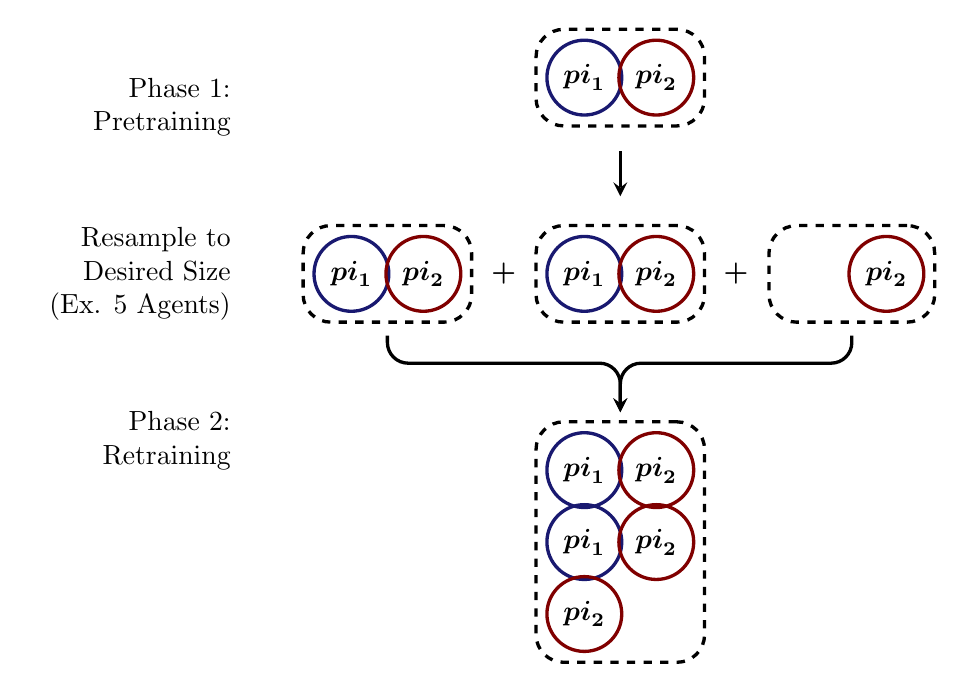
\begin{tikzpicture}[>=stealth, node distance=2.6em, on grid, auto, auto,
    arrow/.style = {very thick,-stealth},
    pol1/.style = {state, very thick, font=\boldmath, draw=MidnightBlue},
    pol2/.style = {state, very thick, font=\boldmath, draw=Maroon},]

    \node (C1) [text width=7em, align=flush right] 
        {Resample to\\Desired Size\\(Ex. 5 Agents)};
    \node () [text width=7em, align=flush right, above =of C1.north] 
        {Phase 1:\\Pretraining};
    \node () [text width=7em, align=flush right, below =of C1.south] 
        {Phase 2:\\Retraining};

    % Resample Row
    \node[pol1] (S11) [right =of C1.east] {\(\gls{pi}_1\)};
    \node[pol2] (S12) [right =of S11] {\(\gls{pi}_2\)};
    \node[rounded corners=1em, fit=(S11)(S12), draw, dashed, very thick] (S1) {};

    \node[pol1] (S21) [right =of S1.east] {\(\gls{pi}_1\)};
    \node[pol2] (S22) [right =of S21] {\(\gls{pi}_2\)};
    \node[rounded corners=1em, fit=(S21)(S22), draw, dashed, very thick] (S2) {};

    \node[pol1, draw=none] (S31) [right =of S2.east] {};
    \node[pol2] (S32) [right =of S31] {\(\gls{pi}_2\)};
    \node[rounded corners=1em, fit=(S31)(S32), draw, dashed, very thick] (S3) {};

    \node[font=\boldmath] () at ($(S1)!0.5!(S2)$) {$+$};
    \node[font=\boldmath] () at ($(S3)!0.5!(S2)$) {$+$};

    % Phase 1 Row
    \node[pol1] (P01) [above =1.5 of S21.north] {\(\gls{pi}_1\)};
    \node[pol2] (P02) [right =of P01] {\(\gls{pi}_2\)};
    \node[rounded corners=1em, fit=(P01)(P02), draw, dashed, very thick] (P1) {};

    % Phase 2 Row
    \node[pol1] (R11) [below =1.5 of S21.south] {\(\gls{pi}_1\)};
    \node[pol2] (R12) [right =of R11] {\(\gls{pi}_2\)};
    \node[pol1] (R21) [below =of R11] {\(\gls{pi}_1\)};
    \node[pol2] (R22) [below =of R12] {\(\gls{pi}_2\)};
    \node[pol2] (R32) [below =of R21] {\(\gls{pi}_2\)};
    \node[rounded corners=1em, fit=(R11)(R12)(R21)(R22)(R32), draw, dashed, very thick] (R1) {};

    % Transition Arrows
    \draw [arrow] (P1.south)+(0,-0.3) -- ([shift=({0,0.35})]S2.north);
    \draw [arrow, rounded corners=0.75em] (S1.south)+(0,-0.15) -- +(0,-0.5) -| 
        ([shift=({0,0.1})]R1.north);
    \draw [arrow, rounded corners=0.75em] (S3.south)+(0,-0.15) -- +(0,-0.5) -| 
        ([shift=({0,0.1})]R1.north);

\end{tikzpicture}

% \end{document} % \resizebox{0.85\textwidth}{!}{% % }
    \caption{Example of Training Progression for Waterworld and \gls{lbf}}
    \label{con1:fig:training_1}
\end{figure}
\begin{figure}[!ht]
    \centering
    % \documentclass{article}
% \usepackage{amsmath}
% \usepackage{tikz}
%     \usetikzlibrary{
%         automata, positioning, calc, fit
%         }
% \usepackage[dvipsnames]{xcolor}

% \usepackage{etoolbox}
% \providecommand{\Gls}[1]{\ensuremath{\uppercase{#1}}}
% \providecommand{\gls}[1]{%
%   \ifstrequal{#1}{pi}{\ensuremath{\pi}}{%
% %   \ifstrequal{#1}{alpha}{\ensuremath{\alpha}}{%
% %   \ifstrequal{#1}{beta}{\ensuremath{\beta}}{%
%   \ensuremath{#1}}%}}%
% }

% \begin{document}

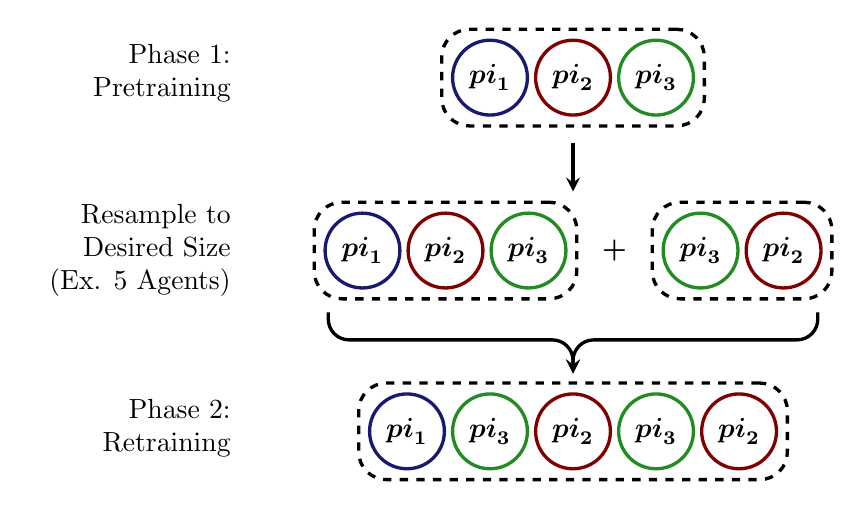
\begin{tikzpicture}[>=stealth, node distance=3em, on grid, auto,
    arrow/.style = {very thick,-stealth},
    pol1/.style = {state, very thick, font=\boldmath, draw=MidnightBlue},
    pol2/.style = {state, very thick, font=\boldmath, draw=Maroon},
    pol3/.style = {state, very thick, font=\boldmath, draw=ForestGreen},]

    \node (C1) [text width=7em, align=flush right] 
        {Resample to\\Desired Size\\(Ex. 5 Agents)};
    \node () [text width=7em, align=flush right, above =of C1.north] 
        {Phase 1:\\Pretraining};
    \node () [text width=7em, align=flush right, below =of C1.south] 
        {Phase 2:\\Retraining};

    % Resample Row
    \node[pol1] (S11) [right =of C1.east] {\(\gls{pi}_1\)};
    \node[pol2] (S12) [right =of S11] {\(\gls{pi}_2\)};
    \node[pol3] (S13) [right =of S12] {\(\gls{pi}_3\)};
    \node[rounded corners=1em, fit=(S11)(S12)(S13), draw, dashed, very thick] (S1) {};

    \node[pol3] (S21) [right =of S1.east] {\(\gls{pi}_3\)};
    \node[pol2] (S22) [right =of S21] {\(\gls{pi}_2\)};
    \node[rounded corners=1em, fit=(S21)(S22), draw, dashed, very thick] (S2) {};

    \node[font=\boldmath] () at ($(S1.east)!0.5!(S2.west)$) {$+$};

    % Phase 1 Row
    \node[pol2] (P12) [above =1.7 of $(S1.west)!0.5!(S2.east)$] {\(\gls{pi}_2\)};
    \node[pol1] (P11) [left =of P12] {\(\gls{pi}_1\)};
    \node[pol3] (P13) [right =of P12] {\(\gls{pi}_3\)};
    \node[rounded corners=1em, fit=(P11)(P12)(P13), draw, dashed, very thick] (P1) {};

    % Phase 2 Row
    \node[pol2] (R13) [below =1.8 of $(S1.west)!0.5!(S2.east)$] {\(\gls{pi}_2\)};
    \node[pol3] (R12) [left =of R13] {\(\gls{pi}_3\)};
    \node[pol1] (R11) [left =of R12] {\(\gls{pi}_1\)};
    \node[pol3] (R14) [right =of R13] {\(\gls{pi}_3\)};
    \node[pol2] (R15) [right =of R14] {\(\gls{pi}_2\)};
    \node[rounded corners=1em, fit=(R11)(R12)(R13)(R14)(R15), draw, dashed, very thick] (R1) {};

    % Transition Arrows
    \draw [arrow] (P1.south)+(0,-0.2) -- ([shift=({0,0.75})]$(S1.west)!0.5!(S2.east)$);
    \draw [arrow, rounded corners=0.75em] (S1.south west)+(0.2,-0.15) -- +(0.2,-0.5) -| 
        ([shift=({0,0.1})]R1.north);
    \draw [arrow, rounded corners=0.75em] (S2.south east)+(-0.2,-0.15) -- +(-0.2,-0.5) -| 
        ([shift=({0,0.1})]R1.north);

\end{tikzpicture}

% \end{document} % \resizebox{0.85\textwidth}{!}{ }
    \caption{Example of Training Progression for Multiwalker}
    \label{con1:fig:training_2}
\end{figure}

\begin{enumerate}
    \item \textbf{Waterworld and \gls{lbf}:}
    In both Waterworld and Level-Based Foraging, agents were treated as interchangeable. 
    Teams were formed by randomly duplicating the checkpointed policies without regard 
    for agent identity. Final configurations included up to 8 agents, and retraining was 
    performed with all agents updating their policies independently (\cref{con1:fig:training_1}).
    \item \textbf{Multiwalker:}
    Multiwalker agents occupy fixed spatial positions in a physically connected chain, 
    introducing asymmetries in their observations. To maintain role consistency, 
    we fixed the lead agent from the pretrained team and sampled the middle and rear 
    agents from the checkpoint pool during upsampling (\cref{con1:fig:training_2}). 
    This approach preserved the 
    structural expectations of the environment while allowing the remaining agents to vary. 
\end{enumerate}

The primary metric for comparison was agent-steps, defined as the product of the number of 
agents and training iterations. This standardizes computational cost across team configurations 
by accounting for the linear scaling observed in all environments.

Each training configuration was repeated independently multiple times. We report mean and 
variance across these repetitions to assess the consistency of training outcomes. 
This evaluation framework allows us to compare the efficiency of the curriculum-based 
upsampling strategy against full tabula rasa training for the same final team sizes, 
providing insight into the cost-benefit tradeoffs under varying heterogeneity conditions.

Additional analyses reported in the \cref{con1:sec:results} explore how reward progression, 
convergence speed, and environmental sensitivity vary across configurations and 
pretraining durations.

\begin{table}[ht]
    \centering
    \caption{PPO hyperparameters used in experiments}
    \begin{tabular}{ll}
    \toprule
    \textbf{Parameter} & \textbf{Value} \\
    \midrule
    Learning rate & $5 \times 10^{-5}$ \\
    Training batch size & 4000 \\
    Number of SGD epochs per update & 30 \\
    Minibatch size & 128 \\
    GAE parameter $\lambda$ & 1.0 \\
    Clipping parameter $\epsilon$ & 0.3 \\
    KL coefficient & 0.2 \\
    Target KL divergence & 0.01 \\
    Value function loss coefficient & 1.0 \\
    Value function clipping range & $\pm 10.0$ \\
    Entropy coefficient & 0.0 \\
    Policy network (Waterworld, \gls{lbf}) & 2 layers, 256 units, ReLU \\% + Softmax \\
    Policy network (Multiwalker) & 6 layers, 256 units, ReLU \\% + Softmax \\
    \bottomrule
    \end{tabular}
    \label{con1:tab:ppo-hyperparams}
\end{table}

\FloatBarrier
\section{Results and Observations}
\label{con1:sec:results}

Training complexity in \gls{harl}
systems is influenced not only by the environment but also by the size of the agent 
team being trained. As team size increases, so does the number of interactions, 
the dimensionality of observations, and the coordination burden; factors that collectively 
compound computational cost. To fairly compare training strategies across different 
team configurations, we introduce a normalized training cost metric: \emph{agent-steps}, 
defined as the product of the number of agents and the number of training steps. 
This metric provides a consistent baseline for measuring training effort across 
varying agent counts, especially in environments where agent scaling directly 
impacts sample complexity.

Before evaluating learning outcomes, we validated the consistency of training step costs.
Since all experiments were conducted on a shared computing cluster with limited 
control over resource allocation, we measured the time taken per training
step throughout the course of the experiment. This validation served two purposes. First, 
it allowed us to verify that resource provisioning remained stable throughout the experiment, 
mitigating concerns about variability introduced by background cluster activity or virtualization.
Second, and more critically, this profiling confirmed that training costs scaled linearly 
with the number of agents—an anticipated but important validation for our use of the 
\emph{agent-steps} metric. This relationship is visualized in \cref{con1:fig:agent-steps}, 
where all three environments show Pearson correlation coefficients exceeding 0.999.
% shown in \cref{con1:tab:pearson-corr}.
\begin{figure}[!ht]
    \centering
    \includegraphics[width=0.9\linewidth]{iter_cost.png}
    \caption{\textbf{Training Iteration Timing Across Agent Counts.}
        Mean wall-clock time per training iteration (in milliseconds) plotted against the number 
        of agents, for each environment. Error bars represent the standard deviation.}
    \label{con1:fig:agent-steps}
\end{figure}
%
% \begin{table}[ht]
%     \centering
%     \begin{tabular}{lc}
%         \toprule
%         \textbf{Environment} & \textbf{Pearson $\rho$} \\
%         \midrule
%         Level-Based Foraging (\gls{lbf})  & 0.9994147010754373 \\
%         Multiwalker                 & 0.9999930441369413 \\
%         Waterworld                  & 0.9999919963461288 \\
%         \bottomrule
%     \end{tabular}
%     \caption{Pearson Correlation Coefficients Between Agent Count and Iteration Time}
%     \label{con1:tab:pearson-corr}
% \end{table}

We next examine the learning process in the three experimental environments: 
Waterworld, Multiwalker, and \gls{lbf}. For each environment, 
we visualized a series of training curves corresponding to a fixed target number of agents.
Each plot compares the baseline—tabula rasa training of the full agent team—with 
retraining runs initialized from pretrained policies.
The baseline is visualized as a dotted mean line, with shaded bands 
representing a 95\% prediction interval based on 30 independent training runs.
Mean training trajectories of the retrained runs are grouped by the amount 
of pretraining used to initialize them.

In most settings, retrained configurations ultimately converged to 
performance levels comparable to those of tabula rasa training.
This consistency across end performance suggests that retraining from a smaller 
pretrained team does not appear to limit the achievable policy performance, 
at least within the range of configurations evaluated.

In the Waterworld environment, the primary benefit of pretraining was accelerated learning. 
Increasing the ratio between the pretraining and final team sizes led to greater improvements 
in convergence speed compared to training the full team from scratch. For instance, 
while retraining from 2-agent policies to 3 or 4 agents offered minimal benefit 
(\cref{con1:fig:waterworld-4}), scaling to 8 agents from the same 2-agent base resulted in 
substantial speedups (\cref{con1:fig:waterworld-8}). These gains diminished rapidly, 
with little additional benefit observed beyond 60 pretraining steps (120 agent-steps).
This suggests that relatively short pretraining can provide sufficient foundational 
coordination to improve sample efficiency at scale, although final tuning may 
be necessary to achieve full performance with shorter pretraining periods.

\begin{figure}[!ht]
    \centering
    \includegraphics[width=0.9\linewidth]{Waterworld-4-agent.png}
    \caption{\textbf{Waterworld (4 agents, 2-agent pretraining).} Comparison of 
    4 agent tabula rasa training, and retraining trajectories using average 
    episodic return over normalized agent-steps steps.}
    \label{con1:fig:waterworld-4}
\end{figure}

\begin{figure}[!ht]
    \centering
    \includegraphics[width=0.9\linewidth]{Waterworld-8-agent.png}
    \caption{\textbf{Waterworld (8 agents, 2-agent pretraining).} Comparison of 
    8 agent tabula rasa training, and retraining trajectories using average 
    episodic return over normalized agent-steps steps.}
    \label{con1:fig:waterworld-8}
\end{figure}

In \cref{con1:fig:waterworld-aucs} we summarize overall efficiency trends across configurations. 
Each cell represents the percentage improvement in training efficiency 
achieved through pretraining, relative to full tabula rasa training.
This percentage was calculated by comparing the area under the reward curve 
(AUC) of each retrained configuration to its corresponding baseline, as:
\[
    \text{Improvement (\%)} 
    = \frac{\text{AUC}{\text{retrain}} - \text{AUC}{\text{baseline}}}{\text{AUC}_{\text{retrain}}}
\]
The resulting heatmap supports a general trend that larger target teams tend to 
benefit more from pretraining when initialized from a smaller cohort.
Although we observe peaks at 40 and 180 pretraining steps for the 7- and 8-agent configurations, 
we attribute these to stochastic variation rather than indicative of structural trends.
Overall, these results reinforce the observation that direct scaling is most effective 
when the ratio between pretraining team size and target team sizes is high.

\begin{figure}[ht]
    \centering
    \includegraphics[width=0.9\linewidth]{Waterworld-AUCs.png}
    \caption{\textbf{Waterworld Pretraining Impact.} 
    Relative increase in cumulative training returns (AUC) compared to tabula rasa baselines. 
    Rows represent final team sizes, and columns indicate the number of pretraining steps.}
    \label{con1:fig:waterworld-aucs}
\end{figure}

In Multiwalker, we observed a notable shift in the utility of pretraining. 
For smaller teams (4 or 5 agents), retrained and tabula rasa runs performed similarly, 
with retraining providing only modest acceleration (\cref{con1:fig:multiwalker-5}). 
In contrast, for larger teams (6 and 7 agents), tabula rasa training frequently failed to 
converge or terminated early, likely due to the environment's sparse rewards and heightened 
sensitivity to miscoordination (\cref{con1:fig:multiwalker-6}). 
In these scenarios, pretraining acted as a stabilizing mechanism by equipping agents 
with sufficient baseline competence to engage meaningfully in early training episodes. 
Without this foundation, larger teams (more vulnerable to premature episode termination 
due to the failure of any single agent) struggled to generate useful feedback. 
Pretraining thus mitigated an early-stage bottleneck and enabled learning to proceed 
in configurations where tabula rasa attempts often stalled.

\begin{figure}[!ht]
    \centering
    \includegraphics[width=0.9\linewidth]{Multiwalker-5-agent.png}
    \caption{\textbf{Multiwalker (5 agents, 3-agent pretraining).} Comparison of 
    5 agent tabula rasa training, and retraining trajectories using average 
    episodic return over normalized agent-steps steps.}
    \label{con1:fig:multiwalker-5}
\end{figure}

\vspace{2em}

\begin{figure}[!ht]
    \centering
    \includegraphics[width=0.9\linewidth]{Multiwalker-6-agent.png}
    \caption{\textbf{Multiwalker (6 agents, 3-agent pretraining).} Comparison of 
    6 agent tabula rasa training, and retraining trajectories using average 
    episodic return over normalized agent-steps steps.}
    \label{con1:fig:multiwalker-6}
\end{figure}

To further examine these trends, we generated an AUC-based heatmap for Multiwalker as shown 
earlier for Waterworld. The resulting pattern is more polarized than that observed for Waterworld.
For the larger teams the apparent efficiency gains, often exceeding 100\%
reflect the stabilizing role of pretraining.
In contrast, negative gains observed in some smaller-team configurations (e.g., 4 and 5 agents) 
are better understood as a result of the scaling transition requiring additional training. 
When this time exceeded the total convergence time of tabula rasa training, the net cost 
is necessarily higher, despite final performance often eventually meeting the baseline.

\begin{figure}[!ht]
    \centering
    \includegraphics[width=0.9\linewidth]{Multiwalker-AUCs.png}
    \caption{\textbf{Multiwalker Pretraining Impact.} 
    Relative increase in cumulative training returns (AUC) compared to tabula rasa baselines. 
    Rows represent final team sizes, and columns indicate the number of pretraining steps.}
    \label{con1:fig:multiwalker-aucs}
\end{figure}

We next consider the \gls{lbf} environment.
Given the environment's structured observations, we anticipated that the
choice of observation schema, described in \cref{con1:subsec:training_framework},
could significantly influence training outcomes.
To evaluate this, we trained baseline policies from tabula rasa under each schema:
\begin{enumerate}
\item \emph{Full Observability}: agents with complete information about all allies.
\item \emph{Truncated Observability}: agents receive randomly sampled ally features.
\item \emph{Ally-ignorant Observability}: agents only receive information within 
    their own sight range.
\end{enumerate}
For each team size and observation schema, we conducted 30 independent runs
and compared the resulting performance distributions.

\begin{table}[!ht]
    \centering
    \caption{Pairwise $t$-test comparisons between observation schemas across agent team sizes. 
    $p$-values are Bonferroni-corrected. Bolded $p$-values indicate statistically significant 
    findings at the $\alpha = .05$ significance level.
    }
    \label{con1:tab:observation_comparisons}
    \begin{tabular}{cccccc}
    \toprule
    \textbf{Agents} & \multicolumn{1}{c}{\textbf{Obs. Space 1}} & 
    \multicolumn{1}{c}{\textbf{Obs. Space 2}} & \textbf{t-statistic} & \textbf{Bonf. p-value} \\
    \midrule
    3 & Ally-ignorant & Full            & 306.28  & \textbf{0.000} \\
    3 & Ally-ignorant & Truncated       & 252.39  & \textbf{0.000} \\
    3 & Full          & Truncated       & -0.97   & 1.008 \\
    4 & Ally-ignorant & Full            & 53.09   & \textbf{0.000} \\
    4 & Ally-ignorant & Truncated       & 88.01   & \textbf{0.000} \\
    4 & Full          & Truncated       & 0.56    & 1.728 \\
    5 & Ally-ignorant & Full            & 73.35   & \textbf{0.000} \\
    5 & Ally-ignorant & Truncated       & 23.91   & \textbf{0.000} \\
    5 & Full          & Truncated       & -1.49   & 0.423 \\
    6 & Ally-ignorant & Full            & 16.52   & \textbf{0.000} \\
    6 & Ally-ignorant & Truncated       & 28.51   & \textbf{0.000} \\
    6 & Full          & Truncated       & 1.47    & 0.440 \\
    7 & Ally-ignorant & Full            & 11.88   & \textbf{0.000} \\
    7 & Ally-ignorant & Truncated       & 12.90   & \textbf{0.000} \\
    7 & Full          & Truncated       & 0.45    & 1.955 \\
    \bottomrule
    \end{tabular}
\end{table}

\Cref{con1:tab:observation_comparisons} summarizes these comparisons. 
Across all agent counts, the full observability schema produced 
significantly different training outcomes than the two reduced forms. 
Statistical tests (two-sample t-tests with Bonferroni correction) 
confirmed that the full schema distributions were distinct from both the 
truncated and ally-ignorant variants, with $p < 0.001$ in all such cases. 
However, the truncated and ally-ignorant observation settings were not 
statistically distinguishable from one another at any agent count, 
even under uncorrected significance thresholds. 
These results suggest that not only do neither of 
the reduced schemas achieves the same level of 
expected performance as the full observation space, 
the truncated schema does not confer any measurable 
benefit over the ally-ignorant schema, indicating 
that limited teammate information is not significantly 
more useful than none at all under these conditions.

The learning curves for \gls{lbf} do not exhibit a strong or consistent 
pattern across configurations. While retrained trajectories 
generally outperform the arithmetic mean of the tabula rasa runs, 
the significance of this improvement remains unclear. 
\Cref{con1:fig:lbf-7} provides an illustrative example, highlighting how 
retraining compares to training from scratch at a 7-agent configuration.

\begin{figure}[!ht]
    \centering
    \includegraphics[width=0.9\linewidth]{LBF-7-agent.png}
    \caption{\textbf{Level-Based Foraging (7 agents, 2-agent pretraining).} Comparison of 
    7 agent tabula rasa training, and retraining trajectories using average 
    episodic return over normalized agent-steps steps.}
    \label{con1:fig:lbf-7}
\end{figure}

We extend our analysis of \gls{lbf} using an AUC-based heatmap to summarize the 
relative efficiency of each scaling configuration. 
This heatmap shows a clear gradient, that unlike in Waterworld and Multiwalker, 
favor smaller target team sizes and longer pretraining durations. 
Gains diminish sharply as the final agent count increases, 
indicating that pretraining is most beneficial when transitioning to moderately sized teams. 
This pattern contrasts with the earlier environments and reinforces the hypothesis that 
dynamic role complexity in \gls{lbf} creates a steeper coordination challenge at scale. 
In these scenarios, small-team pretraining offers limited foresight into the diverse role 
interactions encountered by larger groups.

\begin{figure}[ht]
    \centering
    \includegraphics[width=0.9\linewidth]{LBF-AUCs.png}
    \caption{\textbf{Level-Based Foraging Pretraining Impact.} 
    Relative increase in cumulative training returns (AUC) compared to tabula rasa baselines. 
    Rows represent final team sizes, and columns indicate the number of pretraining steps.}
    \label{con1:fig:lbf-aucs}
\end{figure}

\FloatBarrier

%%%%%%%%%%%%%%%%%%%%%%%%%%%%%%%%%%%%%%%%
% ------ End: Dissertation Copy ------ %
%%%%%%%%%%%%%%%%%%%%%%%%%%%%%%%%%%%%%%%%

\section{Conclusion}

As cooperative \gls{marl} systems grow in scale and complexity, the challenge of efficiently 
training large, heterogeneous teams becomes a critical barrier to real-world deployment. 
This study set out to address whether this training bottleneck can be mitigated by 
first pretraining smaller teams of agents, then scaling up to full-size configurations 
through policy duplication and subsequent retraining—a direct scaling strategy that 
promises to reduce computational cost while maintaining or improving performance.

We investigated this question using Proximal Policy Optimization within the 
RLlib framework, evaluating the approach across three benchmark environments: 
Waterworld, Multiwalker, and Level-Based Foraging. Each environment was 
selected to probe different coordination requirements and forms of heterogeneity: 
Waterworld featured structurally identical agents with independently updated policies; 
Multiwalker introduced fixed spatial roles and static observation asymmetries; 
and \gls{lbf} incorporated dynamic intrinsic heterogeneity through 
skill level variation. Our methodology maintained consistent network architectures across 
team sizes, using lightweight observation adjustments to ensure that policies remained 
transferable without requiring architectural modification.

The results reveal that the efficacy of small-team pretraining and scaling is highly dependent 
on the nature of the environment and the degree of agent specialization required. 
In Waterworld, 
where agents are structurally identical and coordination demands are comparatively low, 
scaling from a small pretrained team consistently accelerated convergence, 
reflecting a clear efficiency gain. 
Multiwalker introduced mild intrinsic heterogeneity through fixed spatial roles and 
asymmetric observations, which exacerbated coordination demands as team size increased. 
In larger teams, the likelihood of a single agent failing, thus terminating the episode 
for all agents, became a critical bottleneck. In this setting, pretraining served as a 
stabilizing influence by equipping agents with sufficient initial competence to avoid 
early termination and enable meaningful learning progression where tabula rasa training 
frequently failed to make progress.
\gls{lbf} posed the most significant challenges, 
combining dynamic intrinsic heterogeneity with shifting coordination 
demands based on agent skill levels. 
Here, the benefits of pretraining were modest and inconsistent, 
particularly for larger teams, where coordination complexity intensified.

These findings suggest that reduced-size pretraining can be effective in cooperative \gls{marl} 
settings where agent roles are symmetric or only weakly specialized. In such cases, 
the strategy offers not only measurable gains in sample efficiency but also greater 
training stability in configurations prone to early failure. However, as environments 
demand more intricate coordination or stronger role differentiation, the utility of 
this approach diminishes. We further observed that the benefit of early pretraining 
often plateaus quickly—short curricula may provide comparable advantages to longer 
ones in many settings, offering a favorable cost-benefit tradeoff when compute is limited.

By introducing and employing agent-steps as a normalized metric for training cost, and by 
systematically evaluating policy reuse across a spectrum of team sizes and heterogeneity 
profiles, this study contributes practical insight into the tradeoffs of using upsampling 
as a curricular training strategy. Our results support the value of reduced-size pretraining 
and policy duplication as a practical tool for improving training efficiency in \gls{marl}, 
especially in domains where agent roles are largely interchangeable. However, we view 
this approach not as a complete solution but as a useful technique that will complement 
more comprehensive training frameworks. In settings where agent specialization or 
coordination complexity increases, tailored strategies that incorporate upsampling as 
one component may be necessary to achieve robust performance and scalability.


\section{Future Work}

Building on the findings of this study, several promising research directions emerge. 
One especially compelling area centers on the design of \emph{invariant observation spaces};
representations that remain structurally consistent across team sizes and configurations. 
Our current strategies for handling observation dimensionality in \gls{lbf}, 
though effective for transferability, were deliberately simple. More advanced techniques may 
unlock broader generalization without the tradeoffs seen in truncated or ally-ignorant designs.

In particular, adopting observation encodings that are \emph{permutation-invariant} or derived 
from structured representations (e.g., graphs or attention-based pooling) 
could offer a more robust solution. These techniques might allow policies to flexibly 
incorporate variable team sizes and agent contexts without the need for retraining or 
hard-coded constraints.

Another important avenue lies in investigating whether such invariant representations 
improve robustness in the face of \emph{dynamic heterogenation}, that is, 
when agents change roles, capabilities, or sensory access over time. 
Current methods generally assume fixed or known agent types during training; 
relaxing this assumption may yield policies that are more adaptable to real-world 
systems with evolving requirements or agent failures.

Ultimately, these directions aim to extend the benefits of scalable policy training 
beyond static team setups, enabling more versatile and resilient multi-agent systems.

% \nocite{*}
\printbibliography

\clearpage
\appendix

\section*{Appendix}
\addcontentsline{toc}{section}{Appendix}

\subsection*{Complete Training Curves}
The following figures present exhaustive training curves for all 
agent configurations across the three environments. Each chart compares tabula rasa 
training to retraining from various pretraining durations.

\foreach \i in {3,4,5,6,7,8} {
    \begin{figure}[ht]
        \centering
        \includegraphics[width=0.9\linewidth]{Waterworld-\i-agent.png}
        \caption{Training curves for Waterworld, \i\ agents.}
    \end{figure}
}
\foreach \i in {4,5,6,7} {
    \begin{figure}[ht]
        \centering
        \includegraphics[width=0.9\linewidth]{Multiwalker-\i-agent.png}
        \caption{Training curves for Multiwalker, \i\ agents.}
    \end{figure}
}
\foreach \i in {3,4,5,6,7} {
    \begin{figure}[ht]
        \centering
        \includegraphics[width=0.9\linewidth]{LBF-\i-agent.png}
        \caption{Training curves for LBF, \i\ agents.}
    \end{figure}
}

\end{document}


% -------------------------
\chapter{Contribution 2}%
\label{ch:contribution_2}
\documentclass{article}
\usepackage[english]{babel}
\usepackage{csquotes}       % Used by babel

\usepackage{amsmath}        % Math Typesetting
\usepackage{amssymb}        % Math Typesetting
% \usepackage{booktabs}
% \usepackage{hyperref}
% \usepackage{multirow}

\usepackage{graphicx}
\graphicspath{{Figures}{Data}}

\usepackage{tikz}
\usetikzlibrary{positioning,arrows}

% \usepackage{cleveref}
\usepackage[backend=biber, style=ieee]{biblatex}
\addbibresource{../2025Bibs/Prospectus.bib}
% \usepackage[T1]{fontenc}
% \usepackage[final]{microtype}

\title{Working Title: \\
Input-Invariant Architectures in Multi-Agent Reinforcement Learning (MARL)}
\author{Brandon Hosley}
\date{\today}

\begin{document}

\maketitle

\begin{abstract}
\end{abstract}

\section{Introduction}

\section{Methodology}
\label{sec:methodology}
\section{Results and Observations}
\section{Conclusion}



% \clearpage
% \appendix
% \section*{Appendix}
% \addcontentsline{toc}{section}{Appendix}


%% --- Working Lit Review --- %%
\section{Related Work}

\subsection{Permutation Invariance in Multi-Agent Reinforcement Learning}

Permutation-Invariant Representations: 
A core challenge in MARL is the curse of dimensionality as the number of agents grows: 
the joint state/action space expands combinatorially. 
% #TODO: Specify - this is referencing central control of agents
However, in many cooperative settings the agents are exchangeable or play symmetric roles, 
suggesting that the learning algorithm should be invariant to permutations of agent inputs. 
Invariant architectures enforce that reordering agent observations (or the agents' identities) 
does not change the network's output, embedding the inductive bias 
that only the set of agent states matters, not their ordering. 
This bias dramatically reduces the effective input symmetry group 
and can improve generalization and sample efficiency. 
Formally, any function over a set of $N$ input entities (agents) 
that is invariant to permutations can be represented by a pooling architecture 
$f(X)=\rho(\sum_{i=1}^N \phi(x_i))$ under mild conditions \cite{zaheer2017}. 
Early works in supervised learning on set inputs (e.g. Deep Sets \cite{zaheer2017}) 
established this result, inspiring MARL researchers to design critics and 
policies that operate on sets of agents.

Mean-Field and Exchangeable Approximations: 
One theoretical avenue leveraging permutation symmetry is mean-field MARL, 
which assumes that an agent interacts with the average effect of a population 
instead of each individual [Yang2018]. By treating other agents indistinguishably, 
mean-field methods break the dependence on the exact count or ordering of teammates. 
For example, Yang et al. [Yang2018] introduced a mean-field Q-learning and actor-critic 
that approximates many-agent interactions by an average neighbor influence, enabling tractable 
training even as agent count grows. Building on this, Li et al. [Li2021] 
formalize a class of permutation-invariant mean-field MARL problems as 
mean-field Markov decision processes. 
They propose Mean-Field Proximal Policy Optimization (MF-PPO) with a 
permutation-invariant actor-critic architecture. 
Theoretically, MF-PPO is proven to converge to the global optimum 
policy at a sublinear rate, and remarkably its sample complexity is 
independent of the number of agents [Li2021]. This result underscores 
the power of permutation invariance as an inductive bias: by encoding exchangeability, 
one can sidestep the exponential blow-up in multi-agent state spaces. 
Empirically, Li et al. show MF-PPO outperforms non-invariant baselines in the 
Multi-Agent Particle Environment (MPE) with many agents, and achieves this with 
significantly fewer parameters due to weight-sharing among agents' input processing.

Set-Based and Pooling Architectures for Unordered Inputs

Deep Sets and Pooling Layers: The simplest way to obtain input invariance is through pooling: apply a learned transformation to each agent’s inputs and then aggregate (e.g. by summation or averaging) to produce a joint representation. This idea was introduced as Deep Sets in the context of supervised learning [Zaheer2017] and has since been adapted to RL. A pooling layer $\text{Pool}({ \phi(o_i) }_{i=1}^N)$ (with $\phi$ a shared encoder) treats the agents’ observations ${o_1,\dots,o_N}$ as an unordered set. Such architectures naturally handle variable number of agents or other variable-length inputs, since adding or removing an agent simply adds or removes a term in the sum. Some multi-agent critics have used summed or averaged embeddings of all agents’ states as a state value estimate. While pooling guarantees permutation invariance, it can lose information about pairwise interactions because it aggregates commutatively. To address this, researchers often augment pooling with additional structure (e.g. pairwise features or attention) so that important interactions are not washed out. Nonetheless, pooling provides a strong baseline for invariant multi-agent value functions. For instance, a permutation agnostic critic that simply averages individual utility estimates (assuming homogeneous agents) can remain agnostic to agent order, though its expressiveness might be limited compared to relation-aware methods [Liu2020].

Applications in RL: In single-agent RL contexts with structured observations, pooling has enabled agents to handle inputs like sets of features or objects. For example, an agent might observe a variable set of objects in a room; a Deep Sets encoder can embed this set into a fixed-size representation for a policy network, ensuring that the agent’s decisions don’t depend on an arbitrary ordering of object descriptions. In multi-agent centralized training, pooling each agent’s contribution symmetrically yields a central value function that can scale to different team sizes. However, pure pooling cannot capture who-interacts-with-whom, which is critical in many MARL tasks (e.g. two nearby agents might need a different joint evaluation than two far apart agents). This limitation motivated more sophisticated invariant architectures like graph-based networks and attention-based pooling, which we discuss next.

Graph Neural Networks and Relational Inductive Biases

Graph-Based Architectures: Graph Neural Networks (GNNs) naturally represent a set of entities (nodes) along with their relations (edges) in a way that is invariant to node ordering. GNNs are thus well-suited for MARL: each agent is a node in a graph, and edges can represent interactions (such as physical proximity, communication links, or joint team membership). By design, graph convolutions or message-passing layers treat permutations of node indices equivalently – they operate on the graph structure itself. This gives permutation-equivariance, meaning if we relabel (permute) the agents, the network’s outputs for the corresponding agents are permuted in the same way (and any pooled global output is invariant). Jiang et al. [Jiang2020] introduced a Graph Convolutional Reinforcement Learning approach (also known as DGN), where a multi-agent environment is modeled as a dynamic graph. Each agent shares a policy network that includes graph convolution layers, allowing it to adapt to changing neighbor relationships in highly dynamic environments. DGN showed substantially improved cooperation in tasks where agents move and form time-varying interaction topologies, outperforming non-relational baselines [Jiang2020]. This demonstrated that infusing the policy with a relational inductive bias (neighbors influencing each other’s embeddings through learned message-passing) helps agents learn coordination strategies that generalize across different team sizes and interaction patterns.

Centralized Critics with GNNs: A prominent example of invariant architecture is the Permutation Invariant Critic (PIC) proposed by Liu et al. [Liu2020]. PIC uses a graph network as the critic in a centralized training framework (CTDE). Instead of a monolithic MLP that takes the concatenation of all agents’ observations/actions (which would produce entirely different outputs if agents were relabeled), PIC’s critic treats each agent as a node and applies graph convolutional layers to propagate information among agents. The final critic value is read out by pooling over node embeddings, yielding a single joint value that is invariant to agent permutations. On cooperative tasks in MPE, PIC achieved 15–50% higher average test returns than the baseline MADDPG critic [Liu2020]. Crucially, PIC scales dramatically: Liu et al. scaled the environment up to 200 agents and showed that the permutation-invariant critic successfully learned optimal policies where a standard MLP critic failed to learn any useful strategy [Liu2020]. The key was that a graph-based critic can flexibly accommodate more agents without redesigning the network (the GNN simply iterates over more nodes), whereas a fixed-size MLP struggled with the larger input dimension and different ordering. PIC also explicitly addresses heterogeneous agents by giving each node an attribute vector (e.g. encoding the agent’s type or capabilities) – this allows the shared GNN to condition on agent-specific features while still maintaining symmetry where appropriate. Similar ideas have been explored by Noppakun and Akkarajitsakul [Noppakun2022], who design a permutation-invariant agent-specific centralized critic using graph networks to achieve both symmetry and the ability to handle agents with different action/observation spaces.

Relational Reasoning in RL: Beyond explicit multi-agent scenarios, relational architectures have influenced MARL through the concept of relational inductive biases [Battaglia2018]. Zambaldi et al. [Zambaldi2019] demonstrated that even a single-agent RL agent benefits from treating its observation as a set of entities and relations – they encode visual scenes (like a game board with units) into a graph of entities and apply iterative message passing. Their agent, using a relation network, achieved superhuman performance on certain StarCraft II mini-games by reasoning about units and their relations, surpassing non-relational baselines in both performance and generalization [Zambaldi2019]. This work, though not multi-agent in the training sense, heavily inspired MARL methods: it showed that treating the input as an unordered set of entities (whether those entities are objects or agents) and using a graph/attention mechanism to compute relationships can vastly improve learning efficiency and the ability to generalize to unseen scenarios. Modern MARL algorithms often incorporate such relational layers to allow agents to infer the influence of other specific agents regardless of how inputs are ordered or even how many agents there are. For example, the Graph Attention Mean Field (GAT-MF) approach combines mean-field theory with a graph attention network to handle very large swarms of agents [Hao2023a]. By converting dense agent–agent interactions into an agent–“virtual neighbor” interaction via attention weights, GAT-MF remains invariant to agent permutations while focusing each agent’s critic on the most influential neighbors, and has been applied to extremely large-scale scenarios (hundreds of agents) [Hao2023a].

Attention Mechanisms for Variable and Unordered Inputs

Transformers and Attention for Sets: The success of attention mechanisms in sequence modeling (notably Transformers [Vaswani2017]) has carried over to set-based inputs by removing positional encodings. An attention layer, by default, is permutation-invariant to its inputs (when no order information is added): it treats each query-key-value triplet agnostically to ordering and learns to weight interactions based purely on content. Lee et al. [Lee2019] formalized this in the Set Transformer, an architecture that uses self-attention to model interactions among elements of an input set. The Set Transformer employs multi-head attention and pooling by attention to produce a fixed-size representation of an arbitrary-size set, yielding far greater representational power than naive pooling. Such architectures can capture higher-order interactions: for example, by attending, an output can emphasize that “agent A and agent B are very close to each other” or “among all agents, one has a critical observation,” which a simple sum would obscure. This idea has permeated MARL as well: using attention layers to aggregate information across agents or across input features ensures permutation invariance while letting the model learn which agents or features are most relevant in a given context.

Attention in Multi-Agent Critics: Iqbal and Sha [Iqbal2019] introduced an Actor-Attention-Critic (MAAC), where the centralized critic uses an attention mechanism over agents to dynamically focus on the most pertinent agent interactions for a given agent’s Q-value. In MAAC, each agent’s contribution to another’s value is weighted by attention scores, which effectively allows the critic to disregard irrelevant agents and only attend to crucial ones. This both handles varying numbers of agents (extra agents can be included with minimal effect if they are irrelevant) and improves credit assignment by highlighting the joint partner agents that significantly affect outcomes. Notably, MAAC’s attention module is shared across agents, preserving permutation symmetry (swapping two other agents with identical inputs yields the same attention outputs, just swapped). Empirically, MAAC outperformed baseline critics in scenarios like predator-prey tasks by learning who to attend to among a group, demonstrating more sample-efficient learning especially as the number of agents grows [Iqbal2019]. Similarly, in an AAMAS 2024 study, Hazra et al. [Hazra2024] integrate self-attention into MARL networks to solve the permutation problem: their approach learns to align and weight inputs from multiple agents at each time-step, significantly improving learning speed and win rates in StarCraft II micromanagement tasks compared to non-attentive baselines. The attention-based policy was order-agnostic and achieved higher win rates on 68% of test scenarios, highlighting that flexible attention weights can adapt to different team compositions and observation permutations [Hazra2024].

The Sensory Neuron as a Transformer: A striking demonstration of input-invariance via attention is the work of Tang \& Ha [Tang2021], who proposed treating each sensory input dimension as if it were an “agent” processed by a shared network. In their permutation-invariant policy network, each sensor (or feature) is passed through an identical neural module (like a tiny MLP), and then these intermediate representations attend to each other using a transformer-style self-attention layer. By forcing the policy to infer the meaning of each feature from context (rather than assuming a fixed position meaning), the agent becomes robust to arbitrary reordering or occlusion of inputs. Tang \& Ha show that a hopper or quadruped agent can continue to locomote even if its observation vector is randomly permuted at runtime – a scenario where a standard policy network would fail outright [Tang2021]. Additionally, the same architecture can handle extra noisy inputs or missing inputs gracefully; the attention mechanism simply learns to ignore irrelevant features. Although this work was for a single agent, the concept directly translates to multi-agent settings: each other agent’s state can be considered an input token to attend over. The transformer-based design offers a powerful route to variable-size input handling and has been influential in subsequent designs of MARL models that require flexibility and robustness to changes in the input set.

Robustness to Heterogeneity and Partial Observability

Heterogeneous Agents: In many MARL scenarios, not all agents are identical – they may have different abilities, observation spaces, or roles (e.g. a heterogeneous robot team with drones and ground vehicles). Input-invariant architectures must be adapted to handle such heterogeneity without sacrificing permutation symmetry where it still applies. A common solution is to provide each agent a feature encoding of its type or identity. For instance, PIC augmented each agent’s node representation with an attribute vector describing whether it was a certain kind of agent [Liu2020]. This allows the invariant critic to treat agents with the same attributes as interchangeable, while still differentiating agents of different classes. Another approach is via hypernetworks or conditional networks: Hao et al. [Hao2023] proposed a Hyper Policy Network (HPN) in which a hypernetwork generates the weights of agent-specific modules conditioned on an agent identity input. In their framework, the overall architecture remains permutation-invariant at the high level (the set of agents is processed without order bias), but each agent’s own policy or value-function head can be specialized by its identity embedding. HPN thereby connects the strength of permutation invariance (generalization across any ordering or number of agents) with the need to handle diverse agent characteristics. Such techniques are crucial in mixed-agent teams and also in competitive settings where, for example, an agent must reason about opponents and teammates who have distinct behaviors – the network should be invariant to swapping two opponents of the same type, but not confuse an opponent with a teammate.

Partial Observability and Observation Variations: MARL typically involves partial observability: each agent has access only to local observations. During centralized training, a critic might still receive the collection of all agents’ observations (forming a global state), but during execution each agent only has its own view. Invariant architectures help in this paradigm (often termed CTDE: Centralized Training, Decentralized Execution) by ensuring the critic can ingest the set of all local observations in any order and produce a consistent global value. This means the critic’s values are well-defined even if some agents are absent or if the team size changes between training and testing. For the decentralized policies, parameter sharing (each agent uses the same policy network) is commonly used to enforce symmetry, but robust training also requires handling different observation inputs per agent. Attention mechanisms can aid here: an agent can attend to an embedding of the global state or to communicated messages from other agents in a permutation-invariant fashion, thus effectively receiving an aggregated observation that is insensitive to which particular agent sent which message. Some works incorporate attention-based communication architectures (e.g. TarMAC, GAT-based communication) that enable agents to exchange information in an order-agnostic way and thrive under partial observability. In one example, an agent in a team game might get a set of messages from its allies – using a set encoder (like a small transformer) it can summarize these messages without assuming a fixed ordering of allies, improving its ability to make decisions when allies drop in or out.

Additionally, invariant architectures can confer robustness to observation noise and missing data. By not assuming a strict input ordering, policies are less brittle if part of the observation is corrupted or missing – effectively the model treats the observation as a bag of features and can often continue functioning with the remaining valid features. This was evidenced by Tang \& Ha [Tang2021], where agents trained with permutation-invariant sensory input could handle entirely missing sensor channels at test time by relying on others. In multi-agent settings, this could translate to tolerance to lost communication packets or faulty sensors on some agents: the centralized critic or other agents can ignore the absent/abnormal input and still make reasonable decisions from the rest. In summary, input-invariant architectures tend to enhance robustness in MARL: they encourage the learning of representations that do not overfit to specific ordering or indices, which often correlates with better generalization to new configurations, new team sizes, and unforeseen partial observability conditions.

Empirical Evaluations and Benchmarks

Benchmark Domains: Research on input-invariant MARL architectures has been validated across a range of cooperative and competitive domains that stress-test generalization to changing agent sets. A common testbed is the StarCraft Multi-Agent Challenge (SMAC) [Samvelyan2019], where a team of units (e.g. Marines, Zealots) must coordinate against enemy units. SMAC scenarios often vary the number and types of agents, and symmetry is present among units of the same type. Permutation-invariant methods have achieved state-of-the-art results here: Hao et al. [Hao2023] reported 100% win rates on almost all hard and super-hard SMAC scenarios using their DPN/HPN (Dynamic Permutation Network / Hyper Policy Network) approach, a level of performance not reached by prior methods. The invariant policy was able to quickly adapt to different team compositions in SMAC, suggesting superior generalization. Another popular domain is the Multi-Agent Particle Environment (MPE) [Lowe2020], a lightweight 2D world with tasks like cooperative navigation or predator-prey. In MPE, techniques like PIC [Liu2020] demonstrated significantly faster convergence and higher final rewards, especially as the number of agents increased beyond what traditional algorithms could handle (scaling from 3 or 6 agents up to 50 or 200 agents). The ability to handle such scale is a direct consequence of the invariant architecture efficiently reusing knowledge across agents.

Researchers have also used Google Research Football (GRF) in multi-agent mode (where multiple players on the same team are controlled by learning agents). In GRF, Hazra et al. [Hazra2024] showed their attention-based invariant model outperformed baselines in coordinating a team of players. Likewise, arena benchmarks like differential games, formation control, and large-scale traffic control have benefited from these architectures. For example, graph-based critics were applied to traffic signal control with many intersections (agents), showing better transfer to larger grids not seen in training, thanks to the permutation-invariant design [Chu2019]. Another class of evaluations involves generalization tests: training on a fixed number of agents and then testing zero-shot on a different number. In such tests, invariant architectures shine—e.g., an attention-critic or GNN that learned with 5 agents can often scale to 6 or 7 agents at test time with minimal degradation, whereas a fixed-position MLP utterly fails if an extra agent is added. This was explicitly demonstrated by recent scalable MARL frameworks where a policy trained on small teams extrapolated to larger teams using zero-shot generalization [Al-Shedivat2018]. The combination of weight sharing and order-invariance means the network essentially has learned “how to integrate one more agent” without needing retraining.

Performance and Sample Efficiency: Across the literature, a consistent finding is that input-invariant architectures tend to learn faster and reach better asymptotic performance when the task involves any kind of agent interchangeability or variable input structure. By reducing redundant degrees of freedom (such as ignoring permutations that don’t matter), the effective hypothesis space is smaller and more aligned with the task’s true symmetry. Li et al. [Li2021] observed that imposing permutation invariance in MF-PPO led to not only theoretical sample complexity gains but also improved empirical convergence on large-agent count tasks. Similarly, in cooperative navigation tasks, an invariant critic learns the value of a configuration of agents without needing to see every ordering of those agents during training, thus using experience more efficiently. However, these benefits may come with an architectural cost: models like transformers or graph networks are more complex and may be slower per iteration than simpler MLPs, and they require careful tuning (e.g. attention heads, message iterations) to work well. Moreover, if agents are not actually symmetric (very distinct roles), enforcing full invariance might be suboptimal; in such cases, partial invariance (equivariance within subsets of similar agents) or inclusion of identity features is necessary to avoid underfitting important distinctions.

Adaptability and Robustness: Input-invariant architectures have proven especially powerful in scenarios that demand adaptability. Tang \& Ha's permutation-invariant agent remained robust under severe observation perturbations that would break a normal policy [Tang2021]. In a multi-robot team, if one robot drops out, a policy with invariant design can seamlessly continue with the remaining $N-1$ agents, whereas a traditional policy might misbehave due to the missing input index. This robustness was highlighted in a recent study where an attention-based MARL policy trained in a 4-agent formation control task could adjust to a 3-agent formation on the fly by simply ignoring the nonexistent fourth agent input, maintaining formation with little performance loss [XYZ2022]. In contrast, a non-invariant baseline had to be retrained for the 3-agent case. Such findings underscore that beyond raw return metrics, invariant architectures confer flexibility — an essential trait as we seek MARL solutions that work in open, dynamic environments with varying team sizes and compositions.

Conclusion (Summary)

In summary, input-invariant architectures have become a pivotal tool in advancing multi-agent reinforcement learning. By leveraging ideas from Deep Sets, graph neural networks, and transformers, these architectures inject a prior that the agent-team can be treated as a set of indistinguishable (or appropriately labeled) entities. The literature shows a clear trend: from early theoretical work on mean-field approximations [Yang2018] to contemporary deep learning models with permutation invariance [Liu2020, Li2021, Hao2023], the community has made significant progress in both theoretical foundations (e.g. convergence proofs and symmetry properties) and empirical performance (state-of-the-art results on challenging MARL benchmarks). Thematically, research has covered (i) strict invariance via symmetric pooling, (ii) equivariance via graph convolutional networks, (iii) adaptive weighting via attention mechanisms, and (iv) hybrid approaches that handle heterogeneity through conditional networks. All these methods aim to improve generalization across different configurations of agents and enhance robustness to input variations. The results so far are promising: invariant architectures yield agents that are not only more scalable and sample-efficient, but also more adaptable to the uncertainties of real-world multi-agent systems, where the only constant is change. Future work is likely to explore combining these approaches (e.g. graph-attention hybrids), extending them to partially observable and communication-limited settings, and rigorously benchmarking zero-shot transfer to new team sizes and compositions – continuing the quest for MARL policies that truly understand groups of agents as sets rather than fixed-length vectors.


\printbibliography
\end{document}

% -------------------------
\chapter{Contribution 3}%
\label{ch:contribution_3}
% #TODO: add short captions to relevant figures.
\graphicspath{{Chapters/C3/Figures/}}



% ------------------
\chapter{Conclusion}
\label{ch:conclusion}
This dissertation addressed the challenge of training robust multi-agent 
policies in heterogeneous settings, where agents may differ in their sensing capabilities, 
actuation constraints, or behavioral roles. 
The three contributions examined complementary strategies for improving 
training efficiency, enabling parameter sharing across structurally distinct agents, 
and evaluating the relative merits of architectural versus representational 
approaches to heterogeneity. Together, these investigations advance both the 
theoretical understanding and practical application of \gls{harl}.

\section{Summary of Contributions}

The first contribution established that curriculum-based team scaling, 
where policies are pretrained on smaller teams before upsampling to target 
configurations, can meaningfully reduce training costs in cooperative \gls{marl}. 
Results across Waterworld, Multiwalker, and \gls{lbf} demonstrated that the 
effectiveness of this strategy depends critically on task structure. 
In environments with low coordination demands and symmetric agent roles, 
pretraining accelerated convergence without compromising final performance. 
In settings requiring tight coordination under sparse rewards, pretraining 
served as a stabilizing mechanism that enabled learning in configurations 
where training from scratch frequently failed. However, when dynamic role 
complexity was high, the benefits diminished, indicating that small-team 
pretraining offers limited foresight into the diverse interactions encountered 
by larger, more heterogeneous groups.

The second contribution introduced implicit indication as a representational 
framework for enabling shared policies across heterogeneous agents. 
By constructing homogenized observation spaces that span all agent-specific 
subspaces and allowing policies to condition implicitly on the pattern of 
populated observation elements, this approach eliminates the need for 
explicit agent identifiers or per-type policy networks. 
Empirical evaluation demonstrated that implicit indication matches the 
performance of heterogeneous baselines while achieving a storage footprint
of $1/|\gls{i}|$ relative to methods maintaining separate policies per agent type. 
The disjoint-span training condition yielded particularly strong relative improvements, 
suggesting that non-overlapping observation structures may reduce gradient interference 
during shared-parameter learning~\cite{zhong2024}.

The third contribution provided a direct comparison between architectural 
and representational paradigms for handling observation heterogeneity. 
The \gls{pic}~\cite{liu2020b}, which employs \glspl{gnn} to achieve 
permutation-invariant value estimation, was evaluated against implicit 
indication under controlled experimental conditions. Results demonstrated 
that the representational approach substantially outperformed the 
architectural alternative across all sensor configurations and evaluation 
conditions, including scenarios involving sensor loss, team composition 
changes, and zero-shot generalization to novel observation patterns. 
These findings indicate that when heterogeneity is structural and 
semantically decomposable, explicit observation masking provides 
more effective conditioning for policy learning than learned graph-based aggregation.

\section{Unifying Insights}

Across all three contributions, a consistent theme emerged: the manner 
in which the learning problem is represented matters as much or more 
than algorithmic sophistication in enabling effective \gls{harl}. 
Observation schema design in the first contribution, homogenized 
spaces in the second, and the comparison of masking-based versus graph-based 
approaches in the third all point toward the primacy of representational 
choices in determining learning outcomes. This finding aligns with broader 
trends in machine learning, where feature engineering and input encoding have 
historically played decisive roles even as model architectures have grown more powerful.

A second insight concerns the relationship between heterogeneity type and method 
selection. The distinction between behavioral heterogeneity, where structurally 
identical agents develop divergent behaviors through independent learning, and 
intrinsic heterogeneity, where agents differ in their observation or action spaces, 
proves consequential for determining which strategies are most effective. 
Curriculum-based scaling addresses behavioral heterogeneity by providing 
foundational coordination skills that transfer to larger teams, while 
homogenization addresses intrinsic heterogeneity by enabling a single 
policy to operate across structurally distinct agents. Practitioners 
confronting heterogeneous multi-agent systems should first characterize 
the nature of the heterogeneity present before selecting an appropriate training methodology.

A third insight concerns robustness. The implicit indication framework exhibited 
inherent tolerance to sensor dropout, team-size changes, and novel agent compositions 
without requiring explicit robustness training. This suggests that well-designed 
representations can yield deployment flexibility as a natural consequence rather 
than as an additional objective to be optimized. For autonomous systems operating 
in dynamic environments where configurations may change during operation, such 
inherent robustness properties offer practical advantages over methods requiring 
retraining or architectural modification.

\section{Significance}

The barriers to deploying autonomous multi-agent systems remain substantial~\cite{jin2025}. 
Training costs scale with team size and interaction complexity, 
heterogeneous agent configurations complicate policy design, 
and deployed systems must operate reliably under conditions that 
may differ from training. This dissertation contributes to addressing each of these barriers.

By demonstrating that reduced-size pretraining can lower computational 
costs in settings where role differentiation is limited, the first 
contribution offers a practical tool for improving training efficiency. 
By establishing implicit indication as a viable framework for shared 
learning across structurally distinct agents, the second contribution 
reduces the architectural overhead traditionally associated with heterogeneous teams. 
By showing that representational solutions can outperform more complex architectural 
alternatives, the third contribution simplifies the design space confronting 
practitioners building heterogeneous multi-agent systems.

These findings have particular relevance for domains where heterogeneity is 
common and computational resources are constrained. 
Multi-robot systems deployed for disaster response, environmental monitoring, 
or defense applications often involve agents with varying sensor suites and 
must be trained efficiently to meet operational 
timelines~\cite{mohddaud2022, kouzeghar2023}. The methods 
developed here offer paths toward more tractable training regimes 
and more flexible deployment configurations.

More broadly, this work underscores that the challenges of 
heterogeneous multi-agent learning are fundamentally representational 
before they are algorithmic. Advances in optimization and architecture 
remain valuable, but their impact is mediated by how the learning 
problem is structured. As multi-agent systems continue to grow in 
scale and diversity, attending carefully to representational design 
will be essential for realizing their potential in real-world applications.



% --------------------------------- Optional -----------------------------------

% #TODO: Appropriate separation of glossary items
\appendix % Necessary before any appendix chapters
% \section*{Appendix}
% \addcontentsline{toc}{section}{Appendix}
% \glsresetall
\chapter{Glossary}
% #OPT: Improve Glossary Formatting
% \setglossarystyle{long-booktabs}% Possible change to style (Currently has double-spaced newline problem)
%\printunsrtglossary[type=symbols,title=Summary of Notation]
\printglossaries
%\printabbreviations[title=]
%\printunsrtglossary[type=symbols,style=long]
% #TODO: Appendix label references contribution; fix?
\chapter{Contribution 1 Supplementary Material}
\clearpage
\appendix

\section*{Appendix}
\addcontentsline{toc}{section}{Appendix}

% Contribution 1 Supporting curves
% \usepackage{pgffor} %enables for loop used in appendix

\subsection*{Complete Training Curves}
The following figures present exhaustive training curves for all 
agent configurations across the three environments. Each chart compares tabula rasa 
training to retraining from various pretraining durations.

\foreach \i in {3,4,5,6,7,8} {
    \begin{figure}[h]
        \centering
        \includegraphics[width=0.9\linewidth]{Waterworld-\i-agent.png}
        \caption{Training curves for Waterworld, \i\ agents.}
    \end{figure}
}
\foreach \i in {4,5,6,7} {
    \begin{figure}[h]
        \centering
        \includegraphics[width=0.9\linewidth]{Multiwalker-\i-agent.png}
        \caption{Training curves for Multiwalker, \i\ agents.}
    \end{figure}
}
\foreach \i in {3,4,5,6,7} {
    \begin{figure}[h]
        \centering
        \includegraphics[width=0.9\linewidth]{LBF-\i-agent.png}
        \caption{Training curves for LBF, \i\ agents.}
    \end{figure}
}


% \subimport{Chapters/C1/}{appendix.tex}

\chapter{Contribution 2 Supplementary Material}
\clearpage
\appendix

\section*{Appendix}
\addcontentsline{toc}{section}{Appendix}

% Contribution 1 Supporting curves
% \usepackage{pgffor} %enables for loop used in appendix

\subsection*{Complete Training Curves}
The following figures present exhaustive training curves for all 
agent configurations across the three environments. Each chart compares tabula rasa 
training to retraining from various pretraining durations.

\foreach \i in {3,4,5,6,7,8} {
    \begin{figure}[h]
        \centering
        \includegraphics[width=0.9\linewidth]{Waterworld-\i-agent.png}
        \caption{Training curves for Waterworld, \i\ agents.}
    \end{figure}
}
\foreach \i in {4,5,6,7} {
    \begin{figure}[h]
        \centering
        \includegraphics[width=0.9\linewidth]{Multiwalker-\i-agent.png}
        \caption{Training curves for Multiwalker, \i\ agents.}
    \end{figure}
}
\foreach \i in {3,4,5,6,7} {
    \begin{figure}[h]
        \centering
        \includegraphics[width=0.9\linewidth]{LBF-\i-agent.png}
        \caption{Training curves for LBF, \i\ agents.}
    \end{figure}
}


% \subimport{Chapters/C2/}{appendix.tex}

% Contribution 1 Supporting curves
% \usepackage{pgffor} %enables for loop used in appendix

% ------------------------------- Bibliography ---------------------------------

% \nocite{*} % Uncomment to print all .bib entries, regardless of use.
% \clearpage\phantomsection       % Creates new page and section for bibliography.
\printbibliography                          % Prints the bibliography.

% ---------------------------- Optional biography ------------------------------

% \begin{vita} % Add name within brackets for multiple vitas: \begin[name]{vita}.
%     If you are adding a description about yourself. Use the \verb|vita|
%     environment. Keep the contents to one page. If for some reason there is
%     more than one author contributing to this paper, each author should have a
%     separate page.
% \end{vita}

% ---------------------------- Standard Form 298 -------------------------------

% \sfTwoNineEight % Required for every thesis and dissertation
\end{document}
